\documentclass[11pt]{article}
\usepackage[margin=1in]{geometry}
\usepackage{volfit_preamble}
\graphicspath{{figures/}}

\title{\textbf{Three Priors for a Dark Universe}\\[2pt]
\large Graph smile-extrapolation and the assertion dial: smoothness,
contracts, dependencies --- one solver family, three statements about
what the desk is willing to claim\\[2pt]
\normalsize Vol-Fitter Technical Notes, No.~14}
\author{Vol-Fitter}
\date{\today}

% Note-local notation.
\newcommand{\Qsm}{Q_{\mathrm{sm}}}
\newcommand{\Qmsg}{Q_{\mathrm{msg}}}
\newcommand{\QH}{Q_{H}}
\newcommand{\Ldir}{L_{\mathrm{dir}}}
\newcommand{\Arho}{A_{\rho}}

\begin{document}
\maketitle

% Generated numbers. graph_three_priors_tables.tex carries everything unique
% to this edition (gen_graph_three_priors.py); campaign and design-study
% numbers are read from stored artifacts, never re-run.
% Auto-generated by gen_graph_three_priors.py — do not edit.
\newcommand{\gtpabresidual}{-3}
\newcommand{\gtpabbfour}{11}
\newcommand{\gtpabbadafive}{10.0}
\newcommand{\gtpabbadbfour}{14.0}
\newcommand{\gtpsmoothfar}{-3}
\newcommand{\gtpsmoothlitsd}{0.10}
\newcommand{\gtpsmoothfarsd}{1.80}
\newcommand{\gtpsmoothfarsixty}{21}
\newcommand{\gtpthreem}{2.00}
\newcommand{\gtponey}{0.50}
\newcommand{\gtpdeadhalf}{0.40}
\newcommand{\gtppairflat}{1.00}
\newcommand{\gtprepeatvar}{1.67}
\newcommand{\gtpnaivevar}{1.20}
\newcommand{\gtprepeatratio}{1.39}
\newcommand{\gtpcompetecancel}{0.00}
\newcommand{\gtpcompeteout}{-0.50}
\newcommand{\gtpcompetebeta}{0.75}
\newcommand{\gtprhoindex}{0.391}
\newcommand{\gtprhopeer}{0.762}
\newcommand{\gtptwosource}{0.561}
\newcommand{\gtpuplift}{43}
\newcommand{\gtpupliftbar}{15}
\newcommand{\gtpphasen}{1007}
\newcommand{\gtppredtwo}{0.563}
\newcommand{\gtppredgap}{0.3}
\newcommand{\gtphopmean}{1.000}
\newcommand{\gtphopsdgap}{0.0000}
\newcommand{\gtppzero}{1690}
\newcommand{\gtpepst}{0.97}
\newcommand{\gtptauonem}{2.7}
\newcommand{\gtpcalpairs}{11735}
\newcommand{\gtpcallevel}{0.23}
\newcommand{\gtpshaperzero}{0.180}
\newcommand{\gtpshaperone}{0.181}
\newcommand{\gtpclamponem}{3.00}
\newcommand{\gtpclampsd}{1.47}
\newcommand{\gtpsoftthreem}{0.58}
\newcommand{\gtpsoftsd}{1.51}
\newcommand{\gtpdecompsys}{0.82}
\newcommand{\gtpdecompres}{-0.35}
\newcommand{\gtpdecomptotal}{0.47}
\newcommand{\gtpchione}{1.1}
\newcommand{\gtpspecsmoothonem}{0.71}
\newcommand{\gtpspecmsgonem}{0.66}
\newcommand{\gtpspeclayonem}{3.00}
\newcommand{\gtpspecsmoothaapl}{0.28}
\newcommand{\gtpspecmsgaapl}{0.41}
\newcommand{\gtpspeclayaapl}{0.82}
\newcommand{\gtpcycleflags}{0}
\newcommand{\gtpcyclebad}{0.833}
\newcommand{\gtprefagreemsg}{\ensuremath{2.3\times10^{-13}}}
\newcommand{\gtprefagreelay}{\ensuremath{1.0\times10^{-17}}}
\newcommand{\gtprefagreesm}{\ensuremath{1.0\times10^{-17}}}
\newcommand{\gtpcampprior}{286.3}
\newcommand{\gtpcampbase}{279.3}
\newcommand{\gtpcampmsg}{280.9}
\newcommand{\gtpcampmemoryless}{280.2}
\newcommand{\gtpcamphlone}{285.1}
\newcommand{\gtpcamphlfive}{290.1}
\newcommand{\gtpcamphltwenty}{305.5}
\newcommand{\gtpcampdesk}{333.1}
\newcommand{\gtpstressspike}{-14.7}
\newcommand{\gtpstresshigh}{-9.2}
\newcommand{\gtpcalmcost}{+6.2}
\newcommand{\gtpzetahl}{1.68}
\newcommand{\gtpzetabase}{0.74}
\newcommand{\gtpzetamsg}{2.07}
\newcommand{\gtpwingfull}{131}
\newcommand{\gtpwingtransport}{126}
\newcommand{\gtpwingliquid}{193}
\newcommand{\gtpwingliquidtransport}{121}
\newcommand{\gtpcamppairs}{21,958}
\newcommand{\gtpspikeskilllo}{7.9}
\newcommand{\gtpspikeskillhi}{14.2}
\newcommand{\gtphighskilllo}{3.8}
\newcommand{\gtphighskillhi}{7.2}
\newcommand{\gtpcalmskilllo}{0.7}
\newcommand{\gtpcalmskillhi}{0.8}
\newcommand{\gtpidiobefore}{1.91}
\newcommand{\gtpidiobeforetwo}{1.85}
\newcommand{\gtpidioafter}{1.02}
\newcommand{\gtpidioaftertwo}{1.03}
\newcommand{\gtpgencommit}{e2e6c9a}
\newcommand{\gtpgendate}{2026-07-24}


\begin{abstract}
The Vol-Fitter's headline differentiator is filling a mostly-dark universe of
smiles --- one node per $(\text{underlying},T)$ --- from a handful of lit
calibrations.  This note is the account of \emph{how}, told as a choice the
desk must make rather than a single algorithm it must accept.  The production
solver ships three propagation modes, and they are not three tunings of one
idea: they are three different priors, ordered by how much structure the desk
asserts about the dark universe.  \textbf{Smooth field} asserts only
smoothness --- a screened directed-Laplacian Gaussian field, the classical
mathematics of harmonic extension and Tikhonov regularization, the fewest
claims to defend, and the holder of the shipped default by a pre-registered
benchmark gate.  \textbf{Messages} asserts relations --- every edge a
Gaussian contract $z_i\approx\beta z_j$ at a stated precision, the cleanest
static probabilistic semantics in the family: full-amplitude transfer
regardless of confidence, precision-weighted voting, distance taxing
confidence but never the mean, a global information-form solve that never
counts a source twice.  \textbf{Layered} asserts dependencies --- the desk's
native tongue, and the destination of the family: directed influence arcs
cut at the source, a persistent idiosyncratic residual with a half-life,
hard Dirichlet clamps on certified fresh marks, and a reciprocal
beta-harmonic completion --- a prior over \emph{trajectories}, not just
over today's field, flexible up to rigid one-way dependency.  It is the
only prior in the family under which the marks a trader would make by hand
are the marks the solver makes, and the containment is literal: switch off
its directed and temporal layers and what remains \emph{is} the message
operator; decline the contracts too and what remains is the smoothness
belief.  A single asynchronous two-asset story separates the three in four
snapshots: only the layered prior can produce the desk path (a
$\gtpabresidual$-point idiosyncratic dislocation that survives the
source's next tick), and the note derives why the other two \emph{cannot}
--- not as defects, but as exactly the assertions they decline to make.
Every mean-semantics behaviour quoted here runs through the production
solver and is locked by a golden test; every empirical level is read from
stored study artifacts; and the mode question itself is adjudicated by
pre-registered gates whose recorded verdict is quoted honestly: the
layered spatial solve already carries the family's only measured edge in
the stressed regimes --- exactly where books bleed --- while day-old
residual memory does not pay at the one granularity the daily harness can
see, a verdict that prices one dial at one horizon and leaves the mode's
target regime --- intraday asynchrony, the story the note opens with ---
to the pre-registered experiment still open.
\end{abstract}

\newpage
\tableofcontents
\newpage

%======================================================================
\section{A universe, mostly dark}
\label{sec:problem}

The desk owns a universe of smiles, and on any given morning only a few of
them are richly quoted.  The production spine that serves every node is
fixed and worth stating in one breath, because all three propagation modes
live inside it.  Each node receives a \emph{transported prior} baseline
(Note~13's saved prior, moved to today's forward under the spot-dynamics
regime of Note~12, through a strict provenance hierarchy with data-derived
precision tiers); each \emph{lit} node contributes the innovation
$d=\text{calibrated}-\text{transported prior}$ --- a genuine
market-versus-prior move, fitted in pure-market mode; the graph spreads
those innovations to the dark nodes as a posterior increment field
$\widehat z$ with a marginal uncertainty; and each dark node's absolute
handles $h^0+\widehat z$ retarget into Note~01's arbitrage-free smile
machinery, with the functional posterior band and the idiosyncratic ATM
band floor carrying the uncertainty into the drawn smile.  Residual dark
quotes may score a reconstruction afterwards --- never steer it.  The
carrier is the compact handle triple $(\sigma_0,s_0,\kappa_0)$ --- ATM vol,
skew, curvature --- solved as three independent fields.

The interesting question is the middle of that spine: \emph{by what rule do
lit innovations reach dark nodes?}  This note's answer is that there is no
single right rule --- there is a dial.  At one end the desk asserts almost
nothing (``moves are smooth across related smiles'') and receives the
classical mathematics of harmonic extension in return.  At the other end
the desk asserts a full dependency structure (``this name follows that
index, one way, with a beta I will state, and its own dislocations persist
until they decay'') and receives, in return, marks that behave the way a
trader marking by hand would make them behave.  Between the two sits the
contract mode: pairwise relations with stated amplitudes and stated trust,
and nothing more.  The three positions of the dial are the three shipped
propagation modes, they share one seam (same universe, same baselines, same
innovations, same reconstruction), and the fork between them is a single
explicit setting.

\begin{invariant}
\begin{enumerate}[leftmargin=1.6em]
\item A dark node stays at its transported prior unless lit data forces a
move; a component with no active observation path keeps zero innovation,
honestly broad bands, and an explicit flag --- no invented signal, ever, in
any mode.
\item Reported confidence is always the \emph{marginal} posterior
uncertainty, never a conditional; it widens with graph distance and with
informer uncertainty.
\item Amplitude and trust never mix: in every mode, scaling how much a
relation is \emph{believed} must not change how large the implied move
\emph{is} --- trust prices bands, amplitude prices means.
\item One source is one source: however many routes carry it, the solve
prices them jointly --- precision never accrues by path counting.
\item Direction, where asserted, is structural: a layered influence arc is
cut at its source --- no reverse leakage, by construction, not by penalty.
\item The output retargets into the arbitrage-free smile machinery of
Note~01; the graph never emits a raw curve.
\item Mode and default changes are explicit and evidence-gated: the shipped
default is chosen by pre-registered benchmark gates
(\cref{sec:evidence}), and every mean-semantics behaviour in this note is
locked by a golden test against a brute-force reference.
\end{enumerate}
\end{invariant}

\paragraph{Conventions and the notation ledger.}
Node indices $i,j$; the \emph{receiver} of a relation is $i$, its
\emph{informer} (or, in the layered mode, its \emph{source}) is $j$, and
every ordered object reads ``$j$ informs $i$''.  One time symbol $T$
(maturity, years); calendar time within a session is $t$ and an elapsed
interval is $\Delta$.  Innovations $z$ are quoted in the receiving handle's
units; ATM-vol units are scaled so that $0.01$ is one vol point.
Differentiation never appears; all operators are finite-dimensional.  The
three modes share one ledger --- no symbol is reused with a second meaning.

\begin{table}[H]
\centering\footnotesize
\setlength{\tabcolsep}{3pt}
\begin{tabular}{@{}llll@{}}
\toprule
$z,\ d,\ h^0$ & innovations; lit obs.; baseline &
$\beta_{ij},\ p_{ij}$ & relation amplitude; precision\\[2pt]
$\Qsm,\ \Qmsg,\ \QH$ & the three precision operators &
$q_i=\textstyle\sum_j p_{ij}$ & receiver conditional precision\\[2pt]
$\kappa$ & anchor/screen toward zero &
$\alpha_T,\ \rho$ & amplitude shape; class level\\[2pt]
$K,\ \pi$ & trust kernel; mass (\cref{sec:smooth}) &
$g_i$ & gauge/harmonic scale ($\beta_{ij}=g_i/g_j$)\\[2pt]
$u_i,\ \phi_i(\Delta),\ H$ & residual; persistence; half-life &
$W(\Delta)$ & residual process variance\\[2pt]
$m^D_i,\ V^D_i,\ e_i$ & directed prediction; residual meas. &
$\chi_i$ & residual-surprise diagnostic\\[2pt]
$\Omega,\ V_S$ & widened factor cov.; lit covariance &
$r_s,\ p^0_i$ & observation / baseline precision\\[2pt]
$Q^+,\ \Sigma^+,\ G$ & posterior info.; covariance; gain &
$s_i$ & systematic (parent) predictor\\
\bottomrule
\end{tabular}
\caption{Every symbol in the note.  $p$ is always a relation's precision;
baseline precision is $p^0$, never bare $p$; the Kalman-style process
variance is $W$, never $Q$, because $Q$ is reserved for precision
operators.}
\label{tab:ledger}
\end{table}

%======================================================================
\section{A morning's story: the asynchronous pair}
\label{sec:story}

Before any operator is written down, here is the problem the desk actually
has, in the smallest example that contains all of it.  Two assets: $A$ is
liquid and refreshes every unit of time; $B$ is thin.  The desk believes
$B$ follows $A$ one-for-one --- $\beta_{B\leftarrow A}=1$ --- and believes
the influence runs one way: $A$ is the market; $B$ is a satellite.
Snapshots are produced every half unit.  The tape (in handle levels, for
exposition; production runs the identical arithmetic on innovations against
transported baselines):

\[
A:\ 10,11,12,13,14,15\ \text{at}\ t=0,1,2,3,4,5;\qquad
B:\ 10\ \text{at}\ t=0,\quad 10\ \text{at}\ t=3.5 .
\]

What should the published marks do?  Walk it as a trader would.  From
$t=0$ to $t=3$, $B$ is dark and nothing distinguishes it from its
$A$-driven prediction, so it rides the relation: $B$'s mark climbs with $A$
through $10,11,12,13$.  At $t=3.5$, $B$ prints at $10$ while the freshest
$A$ information is its $t=3$ calibration at $13$.  The print is a fact and
must be published unmoved.  It also \emph{teaches} something: relative to
the $A$-driven component, $B$ now carries an idiosyncratic dislocation
\[
u_B \;=\; 10-\beta\cdot 13 \;=\; \gtpabresidual\ \text{points}.
\]
And when $A$ ticks to $14$ at $t=4$ with $B$ dark again, the desk does not
throw that dislocation away: $B$'s mark should be
$\beta\cdot14+u_B=\gtpabbfour$ --- following $A$'s move at full amplitude
\emph{from its own dislocated level}.  The full path is the staircase of
\cref{fig:asyncab}A, and it is worth being precise about its three
load-bearing properties, because each one is an \emph{assertion}, and the
three assertions are exactly what separates the three propagation modes.

\begin{description}[leftmargin=1.7em,style=nextline]
\item[Direction.]  $B$'s surprising print revised $B$'s state only.  The
desk did not mark the S\&P down because one satellite came in cheap; there
is no $B\to A$ channel at all.  This is not a soft preference --- it is a
structural claim: \emph{influence flows one way}.
\item[Memory.]  The $\gtpabresidual$-point dislocation observed at
$t=3.5$ persisted after $B$ went dark again.  A snapshot-by-snapshot
solver, however sophisticated, cannot produce the $t=4$ mark of
$\gtpabbfour$: at $t=4$ its inputs contain no $B$ observation at all.  The
desk is asserting that \emph{an observed idiosyncratic state is part of
today's information}, with its own decay clock.
\item[Rigidity.]  At $t=3.5$ the print was published exactly, and between
prints $B$ tracked $\beta A$ exactly.  The desk asserts the relation at
full force --- conditional on asserting it at all --- and asserts that a
certified fresh mark is a boundary condition, not a suggestion.
\end{description}

\paragraph{Why the memoryless answer is not a smaller version of the same
thing.}  It is tempting to think a static solver merely smooths the same
path.  It does not --- it produces a \emph{different, worse} path, and the
mechanism is instructive.  A symmetric memoryless field solver, run at each
snapshot on whatever is lit at that instant, does three things the desk
just declined to do (\cref{fig:asyncab}B, run through the production
smooth-field solver): at $t=3.5$, with only $B$ lit, the strong $A\!-\!B$
coupling drags the temporarily dark $A$ down toward the satellite's print
($A$'s published mark falls to $\gtpabbadafive$); at $t=4$, with only $A$
lit, the solve has no record that $B$ ever disagreed, so $B$ snaps to
$\gtpabbadbfour$ --- the dislocation is erased by the next source tick; and
both behaviours follow from one root cause: \emph{a joint Gaussian field
conditioned per snapshot has neither direction nor memory}.  Nothing is
broken in the algebra.  The solver answered exactly the question it was
asked --- ``what smooth field explains this instant's lit marks?'' --- and
the desk was asking a different question.

\paragraph{Why no constant beta rescues it.}  Could the desk instead have
wanted a softened path --- say $B=10.5$ at $t=4$, splitting the difference?
Then the $t{=}3.5\to4$ transition requires $10+\beta(14-13)=10.5$, i.e.\
$\beta=0.5$; but continuing to $t=5$ at the same logic,
$10+\beta(15-13)=11.5$ requires $\beta=0.75$.  No constant amplitude
produces both --- the ``softened'' path is not a beta, it is a
\emph{decaying residual}: exactly the mean-reverting state
$u_B(t)=u_B\,2^{-(t-3.5)/H}$ of \cref{sec:layered}, with a finite
half-life $H$.  (A conventional mean reversion $0\le\phi\le1$ can only
make $B$ catch \emph{up} to $A$ faster --- it can never explain a $t=4$
mark below $11$; the flat staircase of \cref{fig:asyncab}A is the
long-half-life limit.)  The same observation kills the tempting
implementation shortcut of measuring $B$'s residual against an
\emph{interpolated} $A$ value at $t=3.5$: interpolating $A$ between $13$
and $14$ uses $A$'s \emph{future} print, and a live system cannot look
ahead.  Causality forces last-tick alignment.

\begin{figure}[H]
\centering
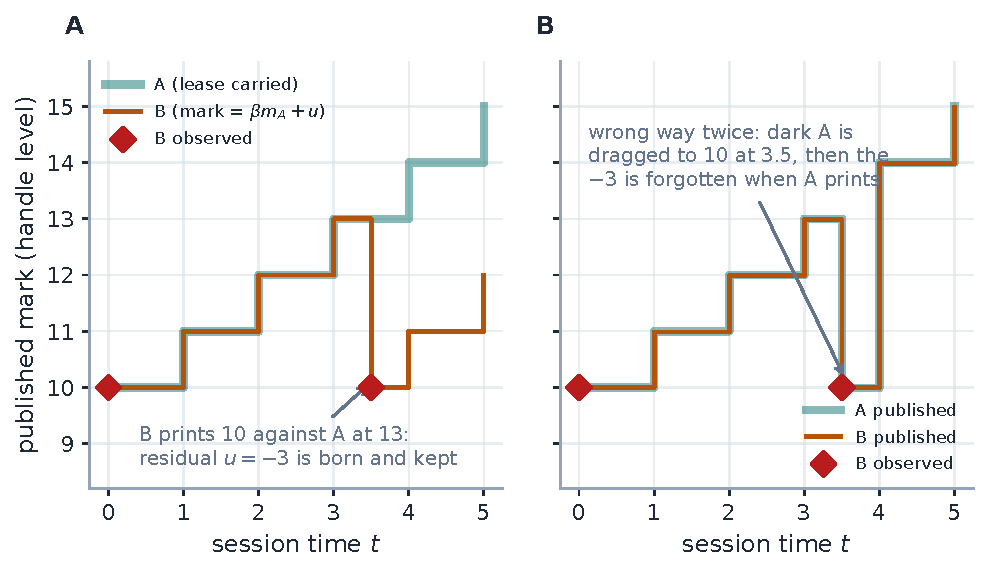
\includegraphics[width=\textwidth]{fig_g3p_asyncab.pdf}
\caption{The asynchronous pair, and the assertion that separates the
modes.  A: the desk path, replayed through the production layered state
machinery (source lease carried flat between prints, hard residual update
at the $t=3.5$ print, dislocation persisting until the next actual $B$
observation) --- the replay reproduces the golden acceptance sequence
exactly.  B: the same tape pushed through the production smooth-field
solver snapshot by snapshot: at $t=3.5$ the satellite's print drags the
dark source down (no direction), and at $t=4$ the dislocation is erased by
the next source tick (no memory).  The second panel is not a bug --- it is
the correct answer to a weaker question.}
\label{fig:asyncab}
\end{figure}

\paragraph{The dial.}  Now the note's organizing claim can be stated
plainly.  The three propagation modes are three priors, ordered by how much
of the story above the desk asserts:

\begin{center}
\footnotesize
\setlength{\tabcolsep}{4pt}
\begin{tabular}{@{}lllll@{}}
\toprule
Mode & Asserts & Mean semantics & Direction & Memory\\
\midrule
Smooth field & smoothness only & emergent & none & none\\
Messages & relations & contractual, exact & symmetric & none\\
Layered & dependencies & contracts $+$ clamps & cut at source &
half-life state\\
\bottomrule
\end{tabular}
\end{center}

Each column purchase has a price.  The smooth field's modesty is why it is
the easiest mode to defend when nothing is configured --- and why its
propagation behaviour is emergent rather than promised.  The message mode's
contracts make every desk sentence a theorem of one static Gaussian --- and
a static symmetric Gaussian is constitutionally unable to express the
story's direction or memory (\cref{sec:messages} derives this, not just
states it).  The layered mode is the only position of the dial that speaks
the whole story, and the other two are its truncations rather than its
rivals: switch off memory, direction and clamps and the layered mode's
reciprocal layer is literally the message operator; decline even the
contracts and what remains is the smoothness belief.  Speaking the whole
story is paid for in state --- persistence brings causality discipline,
invalidation rules, and an adjudication question (``does carried memory
actually predict?'') that \cref{sec:evidence} answers with recorded
numbers rather than enthusiasm.  The next three sections climb the dial in
order of increasing assertion, each with the same contract: say precisely
what is assumed, derive what that buys, and show the production solver
doing it.  Read them as an ascent: each position keeps everything the one
below it earned, and buys back one more property of the desk path.

%======================================================================
\section{Assert smoothness: the smooth field}
\label{sec:smooth}

The first position of the dial asserts the minimum a graph can assert:
\emph{related smiles move similarly}.  No amplitudes are promised, no
directions, no memory --- just a preference for fields that are small and
neighbour-consistent.  The reward for such modesty is that the entire
classical apparatus of smoothing applies, and every object below is a
standard one: a Markov kernel, a Dirichlet-type energy, a screened
Laplacian, a Gaussian-process update.

The desk (or the auto-lattice) supplies raw nonnegative weights, read
``$j$ informs $i$''.  Row-normalization turns them into a row-stochastic
\emph{trust kernel} $K$ ($\sum_jK_{ij}=1$): trust in this mode is
\emph{relative} --- a receiver distributes one unit of attention over its
informers.  A stationary mass $\pi$ ($\pi\T K=\pi\T$) prices each node's
importance in the traffic of the graph.  The increment field then receives
the Gaussian prior $z\sim\mathcal N(0,\Qsm^{-1})$ with
\begin{equation}
\boxed{\;\Qsm=D_\kappa+\eta\,\Ldir^{\beta}+\lambda\,(\Arho+\nu I)^{-1},
\qquad
\Ldir^{\beta}=(I-K\!\circ\!\beta)\T\,\Pi\,(I-K\!\circ\!\beta),\;}
\label{eq:qsm}
\end{equation}
a three-member committee.  The first member, $D_\kappa=\diag(\kappa)$,
charges every node for moving alone --- it is what makes the prior proper,
and it is the same ``anchor toward zero innovation'' object $\kappa$ that
will reappear in both other modes.  The second member charges node $i$ at
its importance $\pi_i$ for the part of its move its informers did not
predict, $z_i-\sum_jK_{ij}\beta_{ij}z_j$: a directed \emph{prediction}
residual, PSD for any real amplitude matrix $\beta$ since it is a Gram
matrix in the $\Pi$-weighted inner product.  The third member (shipped
off, $\lambda=0$) prices a move by the cheapest mass flux that could have
transported it along the graph --- the tangent norm of unbalanced optimal
transport, read through its dual as a screened Poisson problem.  The lit
innovations then condition this prior in covariance form (the
Gaussian-process update, exact, with baseline precision folded in), and
the reported confidence is the reciprocal of the \emph{marginal} posterior
variance --- never the diagonal of the posterior precision, which answers
the wrong (conditional) question and overstates confidence precisely at
the dark nodes whose neighbours are themselves uncertain.

What does this buy?  \Cref{fig:smooth}A shows the production solve on a
calendar chain with one lit node: the innovation propagates outward and
\emph{decays}, the marginal band widening with distance --- with
$\eta$ controlling the reach (\cref{fig:smooth}B): small $\eta$ and the
$\kappa$ member wins (moves stay local); large $\eta$ makes unexplained
neighbour disagreement expensive and the move travels.  This is the
signature smooth-field behaviour, and it is worth contrasting with what is
coming: \emph{decay of the mean with distance is a feature of the
smoothness assertion}, not of graph propagation as such.  (The decay is
not even monotone: at the shipped reach the far node receives essentially
nothing --- \gtpsmoothfar\% of the lit move, a small overshoot below zero,
because the directed residual energy is not an M-matrix interpolant ---
while at $\eta=60$ the transfer reaches \gtpsmoothfarsixty\%.)  The message mode
will make the opposite promise (full amplitude at any distance, with the
band paying the toll), and both promises are internally consistent ---
they answer different questions.

\begin{figure}[H]
\centering
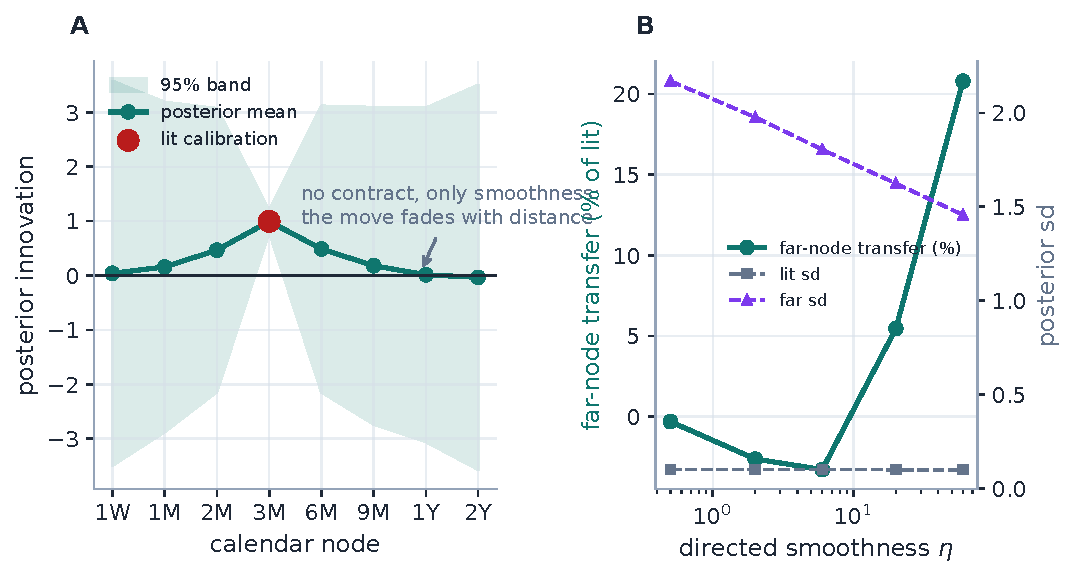
\includegraphics[width=\textwidth]{fig_g3p_smooth.pdf}
\caption{The smoothness prior at work (production solver, eight-node
calendar chain, one lit node at $+1$).  A: the posterior mean decays with
graph distance while the marginal band honestly widens --- essentially
none of the move survives to the far node (\gtpsmoothfar\%, a small
overshoot of zero), the sd growing from \gtpsmoothlitsd\ at the lit node
to \gtpsmoothfarsd\ at the far end.  B: the reach dial: the
directed-smoothness weight $\eta$ sets how expensive unexplained
neighbour disagreement is, and therefore how far a move travels
(\gtpsmoothfarsixty\% at $\eta=60$).  Decay-with-distance is the
smoothness assertion itself, not a law of graph propagation.}
\label{fig:smooth}
\end{figure}

Three honest properties complete the picture, each a direct consequence of
asserting only smoothness.  \emph{Semantics are emergent}: because trust is
row-normalized, adding an informer redistributes attention --- reach,
stiffness and anchoring share coupled dials, and there is no per-relation
sentence of the form ``this edge transfers $+2$ at trust $p$''.
\emph{Inference is symmetric}: the posterior precision is symmetric, so a
satellite's print legitimately pulls an uncertain source --- panel B of
\cref{fig:asyncab} showed exactly this, and within this mode's contract it
is \emph{correct}: absent any directional assertion, evidence flows both
ways.  \emph{There is no state}: the solve is a function of this
snapshot's lit set.  None of these is a defect; each is the absence of an
assertion the desk chose not to make.  And the mode carries the strongest
measured record in the family precisely because it claims so little: on
the stored benchmarks, dark single names behind lit indexes and ETFs gain
$+\gtpspikeskilllo$ to $+\gtpspikeskillhi$ ATM vol bps in the August-2024
spike regime and $+\gtphighskilllo$ to $+\gtphighskillhi$ fully
out-of-sample in the October-2022 bear, with calm-regime skill
$+\gtpcalmskilllo$ to $+\gtpcalmskillhi$ --- never negative --- and
calm-regime dark-name bands made honest by the idiosyncratic ATM floor
($\operatorname{std}\zeta$ \gtpidiobefore$\,\to\,$\gtpidioafter\ and
\gtpidiobeforetwo$\,\to\,$\gtpidioaftertwo).  It is the shipped default,
and \cref{sec:evidence} shows the gate that keeps it there.

\begin{heuristic}
The smooth field is the mode of \emph{least commitment}: a maximum-entropy
flavoured answer to ``I believe these smiles are related but will not say
how much or which way''.  Its mathematics is the oldest and best understood
in the family --- harmonic extension, Tikhonov, Gaussian-process
regression --- which is precisely why it is the right default when no
relation structure has been configured, and the wrong tool when the desk
has a sentence like ``B follows A, one way, beta one'' that it wants
\emph{obeyed}.  It is the ceiling of what an unconfigured solver can know
--- and a desk that never accumulates such sentences is not exercising
modesty, it is leaving information on the table.  The rest of the dial
exists for the day the desk starts talking.
\end{heuristic}

%======================================================================
\section{Assert relations: precision messages}
\label{sec:messages}

The second position of the dial asserts \emph{relations}: for each
configured pair, a sentence with two independent clauses --- how large the
implied move is, and how much the relation is trusted.  The mode's whole
design is that these sentences are \emph{contracts}: every desk-facing
behaviour below is a theorem of one joint Gaussian, locked by a golden
test, and none of them can drift without a named test failing.

\begin{definition}[Message edge]
\label{def:edge}
A relation from informer $j$ to receiver $i$ consists of a conditional
relation precision $p_{ij}>0$, a per-handle amplitude triple $\beta_{ij}$,
and a relation class (calendar, broad index, sector ETF, sector peer,
custom).  Its meaning is the Gaussian statement
\[
z_i=\beta_{ij}\,z_j+\epsilon_{ij},
\qquad \epsilon_{ij}\sim\mathcal N(0,\,1/p_{ij}):
\]
\emph{amplitude says what the receiver's move should be; precision says how
much the relation is trusted.  They never mix.}
\end{definition}

Each relation contributes one rank-one Gaussian factor, and the operator is
their sum:
\begin{equation}
\boxed{\;
\Qmsg=\sum_{(j\to i)}p_{ij}\,u_{ij}u_{ij}\T,
\qquad
u_{ij}=e_i-\beta_{ij}e_j,
\qquad
q_i=\sum_j p_{ij}.
\;}
\label{eq:qmsg}
\end{equation}
Positive semidefiniteness is immediate for arbitrary real betas (a sum of
PSD rank-one terms), and the assembly is sparse by construction --- each
factor touches two nodes.

\begin{proposition}[Receiver conditional]
\label{prop:conditional}
Minimizing the factor energy over $z_i$ with the informers held fixed gives
\[
z_i\mid\{z_j\}\sim\mathcal N\!\left(
\frac{\sum_jp_{ij}\beta_{ij}z_j}{q_i},\ \frac{1}{q_i}\right).
\]
Incoming messages are precision-weighted and \emph{averaged}; independent
incoming conditional precisions \emph{add}.
\end{proposition}

\begin{proof}
The terms of \eqref{eq:qmsg} containing $z_i$ are
$\sum_jp_{ij}(z_i-\beta_{ij}z_j)^2$; completing the square in $z_i$ gives
the stated mean and variance.
\end{proof}

This one line is the entire desk semantics, and \cref{fig:contract} shows
its sharpest consequence through the production solve: on the three-expiry
ladder (3M/6M/1Y, 6M lit $+1$ vol point, $\alpha_T=1$) the dark receivers
land at exactly $\widehat z_{3M}=+\gtpthreem$ and
$\widehat z_{1Y}=+\gtponey$ for \emph{every} edge precision across three
decades, while the posterior standard deviation scales as $p^{-1/2}$.
Amplitude is not a function of confidence --- two dials, because two
fields.  Contrast this directly with \cref{fig:smooth}: where the
smoothness prior made distance decay the mean, the contract prior forbids
it --- along a chain amplitudes multiply while variances accumulate,
\begin{equation}
E[z_C]=\beta_2\beta_1\,E[z_A],
\qquad
\Var(z_C)=(\beta_2\beta_1)^2\Var(z_A)
+\frac{\beta_2^2}{p_1}+\frac{1}{p_2},
\label{eq:hops}
\end{equation}
and \emph{no mean haircut is ever applied for distance}
(\cref{fig:hops}): the mean crosses six hops undamped (production:
$\widehat z=\gtphopmean$ at hop six) while the band pays the toll, the
production marginals matching the accumulation identity to
\gtphopsdgap\ exactly.

\begin{figure}[H]
\centering
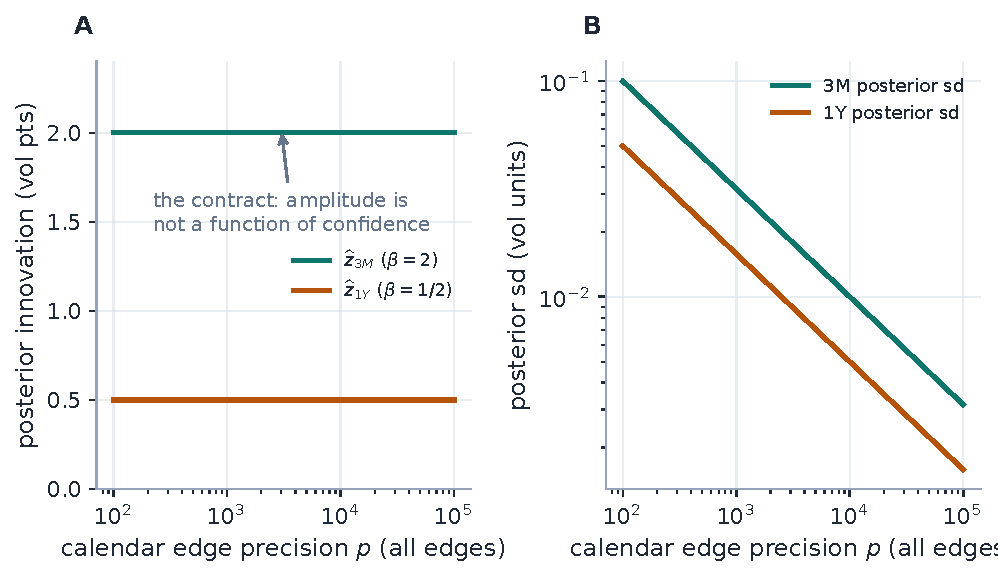
\includegraphics[width=\textwidth]{fig_g3p_contract.pdf}
\caption{The contract, run through the production operator and posterior
(three-expiry ladder, 6M lit $+1$ vol point).  A: the dark receivers'
posterior means sit at the configured amplitudes $+2$ and $+0.5$
regardless of edge precision.  B: what the precision \emph{does} control
--- the posterior standard deviation, falling as $p^{-1/2}$.  Confidence
and amplitude are separate dials because they are separate fields of the
edge.}
\label{fig:contract}
\end{figure}

\begin{figure}[H]
\centering
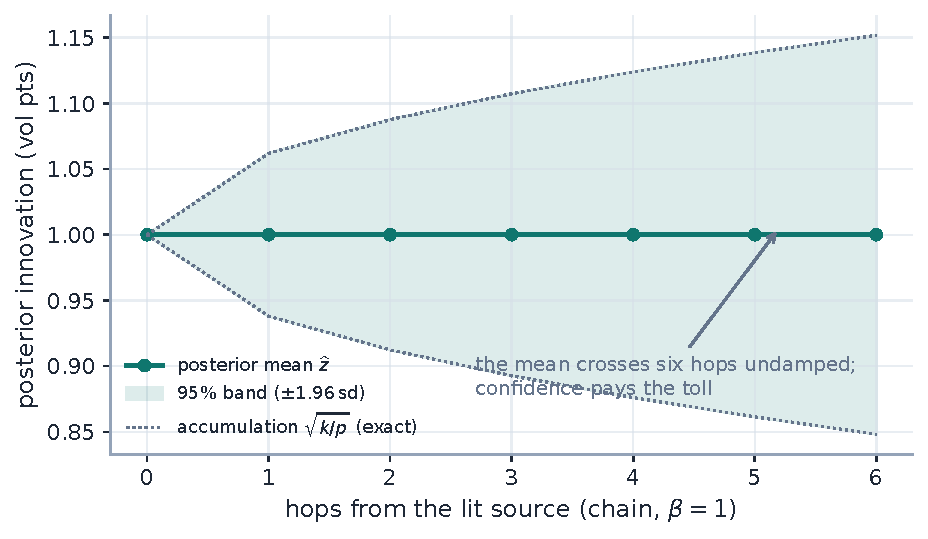
\includegraphics[width=0.88\textwidth]{fig_g3p_hops.pdf}
\caption{Multi-hop propagation under the contract prior (production solve,
six-hop chain, $\beta=1$): the posterior mean crosses every hop undamped
while the marginal band accumulates exactly the per-edge relation
variances of \eqref{eq:hops} (dotted: the closed-form accumulation).
Distance costs confidence, never amplitude --- the exact opposite of the
smoothness prior's signature, and both are correct answers to their own
questions.}
\label{fig:hops}
\end{figure}

\subsection{Why factors, not averages: the dead informer}
\label{sec:rowform}

There is a natural-looking alternative assembly one should examine before
trusting \eqref{eq:qmsg} --- and its failure is the sharpest illustration
of what ``the joint form is a modelling decision'' means.  Normalize each
receiver's incoming precisions into weights $p_{ij}/q_i$ and charge the
receiver once for deviating from its precision-weighted forecast,
$q_i\,(z_i-\sum_j(p_{ij}/q_i)\beta_{ij}z_j)^2$ --- the same shape as the
smooth field's directed residual.  Both assemblies produce the
\emph{identical} receiver conditional of \cref{prop:conditional}, so no
local example can tell them apart.  They differ in the joint distribution,
and the difference has teeth.

\begin{example}[title={Case file: the dead informer}]
\textbf{Setup.}  A receiver hears two informers at equal configured
precision: one lit, one \emph{dead} --- a dark dead-end with no lit path
and no other relations.  What should the lit message transfer?

\textbf{The contract answer.}  Everything: the dead informer carries no
information, so configuring trust in it must cost nothing.  In the
pairwise form this is automatic --- marginalizing an unconstrained
informer removes its factor exactly (the Gaussian integral over a free
$z_j$ of $p\,(z_i-\beta z_j)^2$ is flat in $z_i$) --- and the production
solve transfers \gtppairflat\ of the lit message across four decades of
dead-informer precision (\cref{fig:deadinformer}A), the dead node simply
riding along with a broad marginal.

\textbf{The averaging answer.}  In the row-normalized form the weights are
fixed by \emph{configured} precision whether or not an informer carries
information: the residual can be zeroed for any $z_i$ by moving the free
informer, the posterior is improper, and under a small regularizing anchor
the receiver transfers only \gtpdeadhalf\ of the lit message at equal
precisions --- decaying toward zero as the dead informer's configured
precision grows.  Configuring trust in a silent neighbour \emph{destroys}
a live signal.

\textbf{Two more properties settle the form.}  A reciprocal bidirectional
pair collapses to \emph{one} factor, so auto-generated calendar relations
cannot double-count precision; and the factor list \emph{is} the sparse
assembly --- no normalization couples edges into the same receiver.
\emph{The joint form of an operator is a modelling decision even when
every local conditional agrees.}
\end{example}

The convention that makes one-factor-per-relation well defined is the
\textbf{canonical orientation}: $p\,(z_i-\beta z_j)^2$ and
$p'\,(z_j-z_i/\beta)^2$ are the same factor iff
$p_{j\leftarrow i}=p_{i\leftarrow j}\,\beta^2$ --- the reverse reading of
one contract, in the informer's units.  Auto calendar relations are
therefore quoted with the \emph{shorter} maturity as receiver --- relation
noise in short-dated vol units, where moves are largest and desk intuition
lives --- with implied reverse amplitude $1/\beta$; the receiver
diagnostic $q_i$ maps every incident factor into $i$'s units by the same
identity.  Explicit user relations stay directed as entered; entering both
directions deliberately creates two distinct relations, and the cycle
diagnostics of \cref{sec:accountant} apply.  Note carefully what the
reverse identity says about the dial: \emph{a symmetric factor read
backwards is just as precise} --- a beta-one high-precision contract
between $A$ and $B$ is high-precision in \emph{both} directions.  The
message mode cannot express ``$A$ informs $B$ and never conversely''; the
UI arrow sets units and bookkeeping, not causality.  Where strictly
one-way conditioning is required, the graph must either clamp the source
(only while it is fresh) or move to the layered mode, whose influence arcs
are cut structurally (\cref{sec:layered}).  This is the precise seam
between the second and third dial positions --- and it is a seam, not a
wall: the layered mode's reciprocal layer reuses the message factor
\emph{unchanged} (\cref{sec:harmonic}), so everything configured in this
section --- contracts, precisions, amplitude levels, the gauge --- carries
up the dial intact.  Moving to layered costs nothing already built; it
adds the three assertions this mode cannot make.

\subsection{Amplitude: shape locked, level measured}
\label{sec:amplitude}

For a calendar relation the amplitude is the maturity shape
\begin{equation}
\beta_{i\leftarrow j}=\Big(\frac{T_j}{T_i}\Big)^{\alpha_T},
\qquad \alpha_T=1\ \text{(default, per-handle configurable)},
\label{eq:beta}
\end{equation}
constant total-variance injection --- a $+1$ vol-point move at 6M reads as
$+2$ at 3M and $+0.5$ at 1Y --- and reciprocal by construction:
$\beta_{i\leftarrow j}\beta_{j\leftarrow i}=1$, so a ladder cannot claim
amplification both ways.  On stored data the shape is \emph{weakly
identified} at the day horizon ($R^2$ \gtpshaperzero\ vs \gtpshaperone\
across $\alpha_T\in\{0,1\}$ once the level refits), so $1.0$ is held by
its semantics and the adjudication campaigns sweep it.

Full-force transmission is the correct semantics \emph{conditional on a
relation the desk asserts}.  It is not what the tape does on average: on
$\sim$\gtpcalpairs\ stored adjacent-pair observations the realized
day-over-day calendar transfer under the $\alpha_T=1$ shape is
\gtpcallevel\ per unit of predicted move, and the one-source
index$\to$name transfer is \gtprhoindex.  A default transmitting at full
force would fail the pre-registered RMS gate on its first day.  So
amplitude splits: the \emph{shape} stays locked, and the \emph{level} is a
per-relation-class multiplier $\rho\in(0,1]$ with two presets ---
\texttt{desk} ($\rho=1$, full force, the belief mode) and \texttt{learned}
(the measured levels; they are shape-dependent --- $0.23$ is the
$\alpha_T{=}1$ calendar value, and the $\sqrt T$-shape equivalent is
$0.34$).

How should $\rho$ enter?  Two natural answers are provably wrong.  Scaling
the beta ($\beta\to\rho\beta$) shrinks the forward conditional but
\emph{amplifies} the reverse one by $1/\rho$ --- the reciprocal identity
turns attenuation into amplification.  Emitting two directed shrunk
factors double-counts the relation and composes to
$2\rho/(1+\rho^2)\neq\rho$.  The consistent mechanization of regression
attenuation in both directions of one joint Gaussian is a \emph{local
innovation anchor} --- the $\kappa$ of the ledger, now derived rather than
configured:
\begin{equation}
\kappa_i=p_{\mathrm{primary}}\,\frac{1-\rho_{\mathrm{class}}}
{\rho_{\mathrm{class}}},
\label{eq:anchor}
\end{equation}
with $p_{\mathrm{primary}}$ the largest incident relation precision in
node $i$'s units and $\rho_{\mathrm{class}}$ that primary relation's class
multiplier --- \emph{fixed at build time, never rescaled as further edges
arrive}.  The desk preset $\rho=1$ gives $\kappa=0$ exactly: the belief
mode is the pure contract semantics, not a limit.

\begin{proposition}[Corroboration under the node-linked anchor]
\label{prop:corroboration}
With $k$ equal agreeing clamped sources at precision $p$, beta one, and
the fixed anchor \eqref{eq:anchor}, the receiver's transfer per unit
message is
\[
\frac{kp}{\kappa+kp}=\frac{k\rho}{1-\rho+k\rho}:
\]
one source transfers exactly $\rho$; two lift it to $2\rho/(1+\rho)$;
independent corroboration keeps raising the effective transfer toward one.
\end{proposition}

\begin{proof}
By \cref{prop:conditional} the $k$ agreeing messages average to the common
value at conditional precision $kp$; the anchor adds a zero-innovation
pseudo-message at precision $\kappa$, so the posterior mean shrinks by
$kp/(\kappa+kp)$; substitute \eqref{eq:anchor}.
\end{proof}

The fixed anchor is not a preference; it is the mechanization the data
chose, through a falsifiable prediction.  The alternative --- an
edge-linked anchor $\kappa_i=\sum_jp_{ij}(1-\rho)/\rho$, under which the
transfer is constant at $\rho$ regardless of source count --- predicts
\emph{no} corroboration lift.  The stored benchmark rows adjudicate:
across \gtpphasen\ name-days carrying same-sector peers, the one-source
index transfer slope is \gtprhoindex\ and the measured two-source (index
$+$ peer-average) slope is \gtptwosource\ --- an uplift of
$+\gtpuplift\%$ against a pre-registered $\gtpupliftbar\%$ bar.
Calibrating the fixed-$\kappa$ model on the \emph{single-source slope
alone} predicts \gtppredtwo\ for two sources: agreement to \gtppredgap\%,
with zero free parameters (\cref{fig:amplitude}).

\begin{figure}[H]
\centering
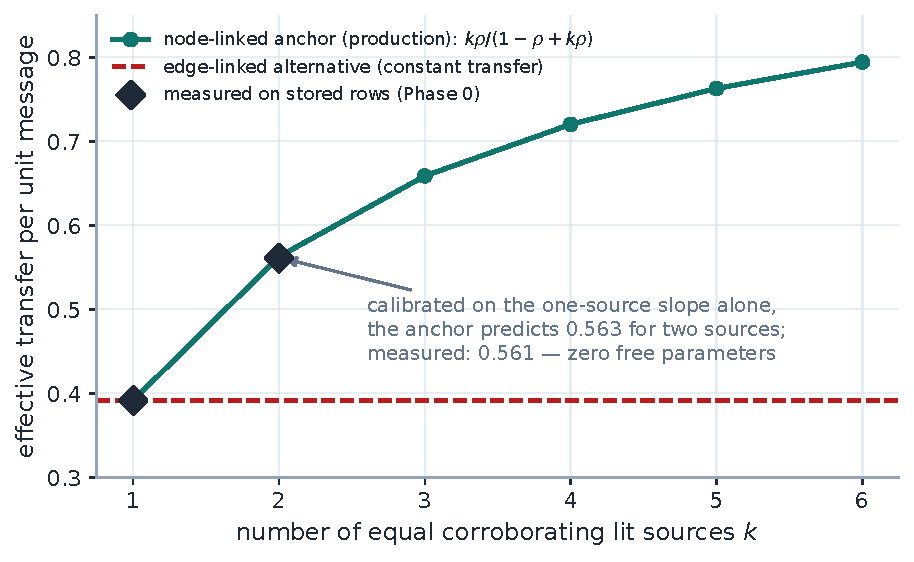
\includegraphics[width=0.9\textwidth]{fig_g3p_amplitude.pdf}
\caption{Amplitude level as a measured object (production anchor and
posterior; measured points from the stored design-study artifact).  The
node-linked fixed anchor produces the corroboration curve
$k\rho/(1-\rho+k\rho)$; calibrated only on the one-source slope
(\gtprhoindex), it predicts the measured two-source transfer to
\gtppredgap\% with no free parameters.  The edge-linked alternative ---
constant transfer regardless of source count (dashed) --- predicts no lift
and is contradicted by the same measurement ($+\gtpuplift\%$ against a
$\gtpupliftbar\%$ bar).}
\label{fig:amplitude}
\end{figure}

\paragraph{Confidence has empirical defaults too.}  The calendar precision
family is
\begin{equation}
p^{\mathrm{cal}}_{ij}
=\frac{p_0}{\epsilon_T+\sqrt{|T_i-T_j|}},
\qquad
p_0\approx\gtppzero\ \text{vol}^{-2},\quad
\epsilon_T\approx\gtpepst\ \sqrt{\text{years}},
\label{eq:calprec}
\end{equation}
with the seeds fitted on the same stored adjacent-pair residuals
(\cref{fig:calendar}B): about \gtptauonem\ vol points of relation noise at
a one-month gap, and --- the honest surprise --- \emph{nearly gap-flat} at
the day horizon: $\epsilon_T$ dominates, the family degrades gracefully
toward constant precision, and whether the decay term earns its keep at
all is one of the campaign ablations (\texttt{constant} and log-distance
families ship beside it).  Cross-class seeds from the same study:
index$\to$name $p\approx1.3\times10^4$, sector peer
$p\approx0.9\times10^4$ (vol units) --- with the recorded caveat that both
are measured on ticker-day \emph{median} innovations and are therefore
upper bounds on per-edge precision.  Two unit disciplines complete the
picture: edge precision is quoted in ATM-vol units, with the skew and
curvature fields scaling it by the squared ratio of the production
per-handle move scales --- a units choice, not a semantics choice, since
the precision-weighted \emph{average} is invariant to a global rescale of
all incoming precisions; and variance is the readable coordinate (an edge
carries $\Var\,\epsilon=1/p$), which is what makes the chain identity
\eqref{eq:hops} legible.

\begin{figure}[H]
\centering
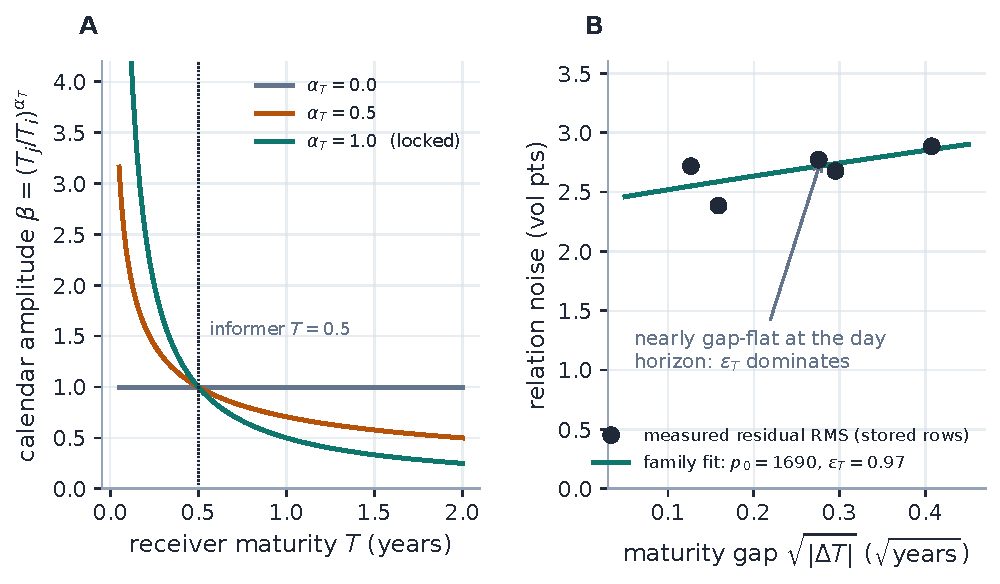
\includegraphics[width=\textwidth]{fig_g3p_calendar.pdf}
\caption{The calendar relation, split into its two fields.  A: the
amplitude shape \eqref{eq:beta} --- what a 6M move implies elsewhere on
the ladder, per exponent; $\alpha_T=1$ (locked) is constant total-variance
injection.  B: the confidence family \eqref{eq:calprec} against the stored
residuals it was fitted on --- relation noise is nearly gap-flat at the
day horizon, so $\epsilon_T$ dominates and the decay term's keep is an
open ablation.}
\label{fig:calendar}
\end{figure}

\paragraph{Exercise 1.}
Derive both rejections of the anchor section: (i) show that replacing
$\beta$ by $\rho\beta$ in one factor turns the implied reverse-direction
amplitude into $1/(\rho\beta)$; (ii) show that two directed factors
$p(z_i-\rho\beta z_j)^2+p'(z_j-\rho z_i/\beta)^2$ with matched units
produce a one-source transfer of $2\rho/(1+\rho^2)$, not $\rho$.  Then
verify from \eqref{eq:anchor} that $\rho=1$ gives $\kappa=0$ exactly.

\subsection{The accountant: the information-form posterior}
\label{sec:accountant}

The factors, the anchors and the lit observations assemble in information
form, solved per connected component of the factor support:
\begin{equation}
\boxed{\;
Q^+=\Qmsg+D_\kappa+H\T R_d H,
\qquad
b^+=H\T R_d\,d,
\qquad
\widehat z=(Q^+)^{-1}b^+,\quad \Sigma^+=(Q^+)^{-1},
\;}
\label{eq:posterior}
\end{equation}
with three honesty rules that are as load-bearing as the algebra.
\emph{No lit path, no invented signal}: components are built on
$\beta\neq0$ edges (a zero-beta factor couples only its receiver --- the
reachability guard that stops an information-free informer from
destabilizing an observed component); a component with no lit observation
is never solved into propriety --- it keeps $\widehat z=0$, the
transported prior, an explicit flag, and an explicitly broad variance;
every observed component is verified positive definite by Cholesky before
inversion.  \emph{Innovations are only as precise as their ingredients}: a
lit innovation is a difference of two estimates, so its observation
precision combines harmonically,
$r^d_s=\big(1/r^{\mathrm{cal}}_s+1/p^0_s\big)^{-1}$, and the placement
rule holds baseline uncertainty to exactly one appearance per node ---
folded into $r^d_s$ for a lit source, added once to the reconstruction
band for a dark node, golden-locked so no node is widened twice.
\emph{Attribution is exact}: the gain matrix $G=\Sigma^+H\T R_d$
decomposes every posterior shift over the observed lit sources,
$\widehat z_i=\sum_sG_{is}d_s$, contributions summing to the shift by
construction --- per independent \emph{source}, never per path, because
path contributions are correlated and non-unique.

The accountant's signature behaviours run through the production solve in
\cref{fig:deadinformer,fig:compete}.  Two routes carrying one source are
priced jointly: on the triangle fixture (source observed at finite
precision $p$, one direct and one two-leg route) the global posterior
variance is $\gtprepeatvar/p$, where naive per-message accounting --- the
\eqref{eq:hops} effective precisions added as if independent --- claims
$\gtpnaivevar/p$, overstating precision by $39\%$.  Competing messages
vote: equal opposing signals cancel to $\gtpcompetecancel$ at
\emph{doubled} conditional precision $2p$ (disagreement is not silence); a
$3p$ source outvotes to $\gtpcompeteout$; and under $\alpha_T=1$ betas the
same $\mp1$ raw signals land at $+\gtpcompetebeta$ --- not a defect but
the contract: signals are mapped into receiver units \emph{before} the
vote, and equal-absolute-vol cancellation is a $\beta=1$ statement.

\begin{figure}[H]
\centering
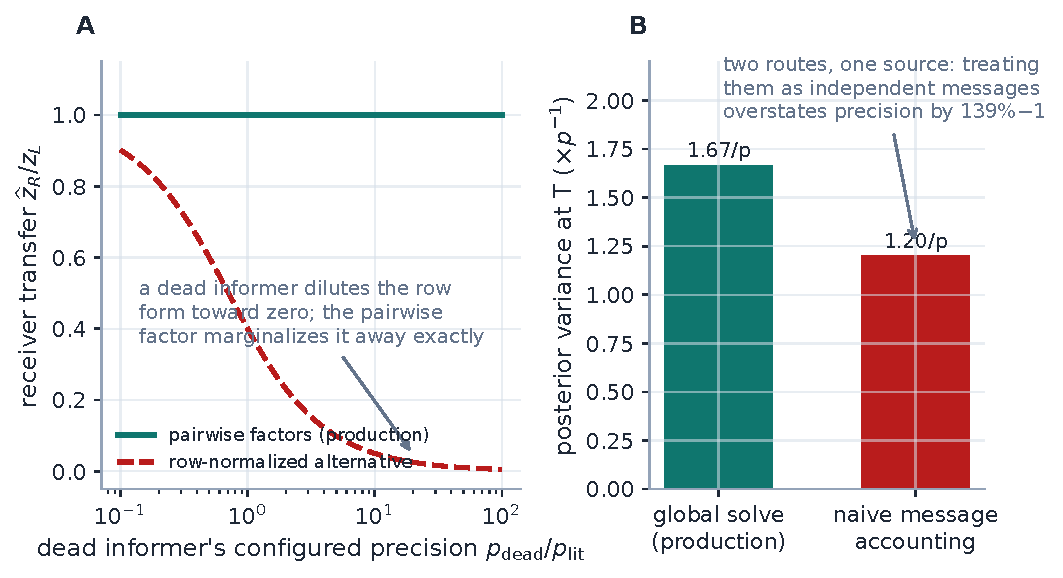
\includegraphics[width=\textwidth]{fig_g3p_deadinformer.pdf}
\caption{The accountant at work (production solves).  A: the dead-informer
case file --- a row-normalized assembly dilutes a lit message toward zero
as a silent neighbour's \emph{configured} precision grows; the pairwise
factor marginalizes the dead informer away exactly.  B: repeated routes
from one source --- the global posterior variance ($\gtprepeatvar/p$)
against naive independent-message accounting ($\gtpnaivevar/p$): path
counting would fabricate a $39\%$ precision overstatement.}
\label{fig:deadinformer}
\end{figure}

\begin{figure}[H]
\centering
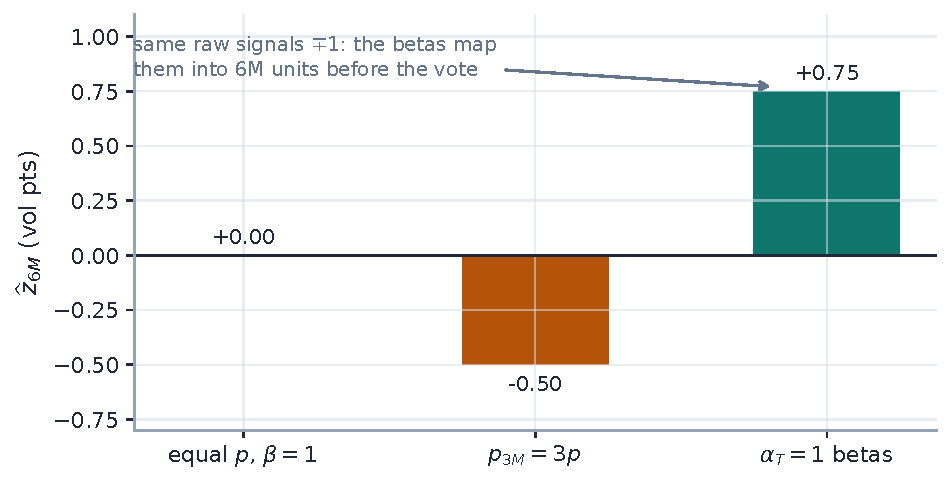
\includegraphics[width=0.88\textwidth]{fig_g3p_compete.pdf}
\caption{Competing messages vote (production solves; 6M dark, 3M and 1Y
lit at $\mp1$ vol point).  Equal precision and $\beta=1$: exact
cancellation at doubled conditional precision.  A $3p$ source outvotes.
Under the locked $\alpha_T=1$ betas the same raw signals map to $-0.5$ and
$+2$ in 6M units before averaging --- the receiver hears receiver-unit
predictions, not raw levels.}
\label{fig:compete}
\end{figure}

Internal consistency of the amplitudes is policed by a gauge argument: a
positive beta structure is cycle-consistent --- every directed cycle's
beta product equals one --- iff there exist node potentials $g_i>0$ with
$\beta_{ij}=g_i/g_j$ (if $\beta_{ij}=g_i/g_j$, every cycle product
telescopes to one; conversely propagate $\log\beta$ along a spanning tree
and any closing edge that disagrees exhibits a bad cycle).  Production
runs exactly this proof as an algorithm --- a union-find sweep with
logarithmic offsets, linear time --- and flags every closing edge whose
implied cycle product strays from one (the reference cross-check of
\cref{app:ref} plants a consistent triangle, zero flags, and an
inconsistent one, flagged at product \gtpcyclebad).  Auto calendar ladders
are gauge-consistent by construction ($g_i=T_i^{-\alpha_T}$) --- and this
same potential-function identity will return in the layered mode as the
change of variables that turns beta-relations into a plain harmonic
problem.

\paragraph{Exercise 2.}
Reproduce panel B of \cref{fig:deadinformer} by hand: with the source
observed at precision $p$ and all three relation precisions $p$, assemble
the $3\times3$ information matrix of \eqref{eq:posterior}, invert, and
show the target's marginal variance is exactly $5/(3p)$, while the
\eqref{eq:hops} effective-message precisions ($p/2$ direct, $p/3$ through
the middle node) sum to $5p/6$, i.e.\ variance $6/(5p)$.  The naive answer
is wrong because both routes share the source's own uncertainty --- the
covariance the global solve refuses to forget.

\paragraph{Exercise 3.}
Three distinct quantities appear at every receiver: edge precision
$p_{ij}$, conditional incoming precision $q_i=\sum_jp_{ij}$, and marginal
posterior precision $1/\Sigma^+_{ii}$.  Construct a two-node example where
$q_i$ is large but the marginal precision is small (an uncertain
informer), and one where the marginal exceeds $q_i$ (the receiver's own
observation).  Only in the idealized clamped-independent-informer case do
the last two coincide --- which is why the wire reports both, and the
desk surface (\cref{sec:universe}) is explicit that ``local $\neq$
final''.

%======================================================================
\section{Assert dependencies: the layered dynamic-harmonic mode}
\label{sec:layered}

The third position of the dial asserts what \cref{sec:story} showed no
static symmetric Gaussian can express: \emph{dependencies}.  Three new
commitments are made, and each buys back one property of the desk path.
Some relations are \emph{influence arcs} --- conditional source-to-target
equations, cut at the source --- rather than reciprocal constraints
(direction).  Each node owns a \emph{persistent idiosyncratic residual}
with its own decay clock (memory).  And a certified fresh calibration is a
\emph{boundary condition} --- its published central value is clamped, not
negotiated (rigidity).  The mode's name describes its architecture: a
directed dynamic \emph{layer} produces predictions that feed a reciprocal
\emph{harmonic} completion, and the two layers own different relation
classes.

It is worth saying plainly why this section is the note's destination.
The three properties of \cref{sec:story} are not preferences a desk might
trade against a basis point of RMS --- they are workflow invariants a
trading book must be able to defend in an audit: a satellite's print must
never mark down the index; a dislocation the desk paid to learn must not
evaporate because the index ticked; a certified fresh mark is a fact, not
a suggestion.  The two priors before this one do not merely \emph{score}
differently against those sentences --- they cannot \emph{state} them.
And the ascent costs nothing already built: every piece of machinery the
note has constructed reappears here as a component --- the message factor
as the reciprocal layer, the gauge potentials as harmonic coordinates,
$\kappa$ as the screen, the accountant's one-source-is-one-source
covariance discipline at the boundary --- so the layered mode is less a
third invention than the family completed: the position of the dial at
which the solver finally speaks the desk's full language.

\subsection{State: the residual and the lease}
\label{sec:state}

The new primitive is the split of a target's innovation into what its
sources explain and what is its own:
\begin{equation}
z_{i,t}=\beta_{ij}\,z_{j,t}+u_{i,t}+\epsilon_{ij,t},
\qquad \epsilon_{ij,t}\sim\mathcal N(0,1/p_{ij}),
\label{eq:directed}
\end{equation}
where $u_i$ --- the \emph{idiosyncratic residual} --- is a state variable
with dynamics
\begin{equation}
u_{i,t+\Delta}=\phi_i(\Delta)\,u_{i,t}+\omega_{i,t},
\qquad
\phi_i(\Delta)=2^{-\Delta/H_i},
\qquad
\omega_{i,t}\sim\mathcal N\big(0,W_i(\Delta)\big).
\label{eq:dynamics}
\end{equation}
Four controls, four different meanings --- and the mode's design
discipline is that they never substitute for one another: $\beta$ is the
mean response to a source move; $p$ is relation noise; $\phi$ (through
the half-life $H$) is how quickly an \emph{actually observed} dislocation
is forgotten; $W$ is how uncertain the residual becomes while unobserved.
Using edge precision to make an old observation fade would conflate
confidence with mean dynamics; using beta to widen uncertainty would
conflate amplitude with confidence; \cref{sec:story}'s constant-beta
computation already showed that no amplitude can imitate a decaying
residual.  The half-life limit $H\to\infty$ ($\phi\equiv1$) is the
random-walk default --- the flat staircase of \cref{fig:asyncab}A --- and
\cref{fig:halflife}A shows the production state object advancing the
$\gtpabresidual$-point dislocation under $H\in\{1,5,20,\infty\}$: what
the desk asserts with $H$ is precisely \emph{how long a private
dislocation is believed}.

Sources carry state too, in a weaker sense: a recent actual calibration
of a liquid name remains the causal source value between expected
refreshes --- an \emph{observation lease}, with a timestamp, a maximum
age, and process variance accumulating since the print.  Two disciplines
make leases safe.  A lease carries the \emph{innovation}, never the
absolute level, so a carried node's published mark keeps moving with its
transported baseline between observations --- carrying levels would
silently break transported-prior semantics.  And a lease is not a saved
output: only states descended from an \emph{actual calibration} are ever
persisted --- graph-predicted values never re-enter as pseudo-data, the
same no-self-feeding invariant every mode obeys, here promoted to a
store-level rule.

\subsection{The directed pass}
\label{sec:directedpass}

With sources resolved (fresh, or carried under lease) and residuals
advanced to the snapshot time, the directed layer sweeps the influence
graph in topological order.  A dark target with parents $P(i)$ receives
the \emph{systematic prediction} and its honest variance:
\begin{equation}
\boxed{\;
m^D_i=\sum_{j\in P(i)}\frac{p_{ij}}{q_i}\,\beta_{ij}\,m_j+m_{u,i},
\qquad
V^D_i=a_i\T\,\Sigma_{P(i)}\,a_i+V_{u,i}+\frac{1}{q_i},
\;}
\label{eq:directedpred}
\end{equation}
where $a_i$ collects the coefficients $(p_{ij}/q_i)\beta_{ij}$ and
$\Sigma_{P(i)}$ is the \emph{full parent covariance}.  That last object
is the implementation's quiet centerpiece: the pass propagates each
node's value as a linear combination of independent \emph{root} variables
(observation innovations, residual states, per-target relation noises),
so the covariance between any two nodes --- including two targets that
share an ancestor --- is exact, by bookkeeping rather than by an
independence assumption.  Two parents carrying the same market factor are
not treated as independent merely because two arcs were configured; the
attribution rows are the same gains, so contributions sum to the mean by
construction, per observed ancestor and per residual, never per path.

Three structural rules complete the layer.  \emph{The cut}: when a target
is observed, its surprise updates the \emph{target's} residual only ---
the pass never writes a parent, so a satellite's print cannot revise the
index, structurally rather than by penalty (golden-locked as zero reverse
influence).  \emph{DAG only}: directed cycles are rejected outright ---
reciprocity is not a cycle's job but the harmonic layer's, and a
topological solve buys exact one-way semantics, no spectral-radius
condition, deterministic order, and transparent attribution.
\emph{Nothing invented}: a dark node with neither supported parents nor a
residual is reported unsupported and stays at its transported prior.

When the target \emph{is} observed, the residual measurement is
\begin{equation}
e_i=d_i-\textstyle\sum_j (p_{ij}/q_i)\beta_{ij} m_j,
\label{eq:resmeas}
\end{equation}
the dislocation of the print against the contemporaneous systematic
prediction --- $10-13=\gtpabresidual$ in the story --- and the state
updates either \emph{hard} (certified prints keep their full dislocation:
$m_u^+=e$, the diffuse-prior limit) or by a finite-quality Kalman step
with gain $K=V_u^-/(V_u^-+V_{\mathrm{obs}}+\beta^2V_j+1/p)$.  One
numerical lesson from building it is worth recording: the posterior
variance must be computed as $K\,r$ (gain times measurement variance),
\emph{not} as the algebraically equal $(1-K)V^-$ --- in the diffuse limit
$V^-\to\infty$ the latter is $\infty\cdot0$ in floating point and
cancels catastrophically; the golden suite caught it.  Either way the
update is cut at the source, and the standardized conflict
\begin{equation}
\chi_i=\frac{d_i-m^D_i}{\sqrt{V_{\mathrm{obs},i}+V^D_i}}
\label{eq:chi}
\end{equation}
is surfaced prominently (\cref{fig:decomposition}B): a loud $|\chi|$
means a genuine idiosyncratic shock, a bad quote, a broken beta, or a
timestamp problem --- the model \emph{keeps} the certified observation
and raises the flag, rather than letting the surprise contaminate the
source.

\subsection{The harmonic completion}
\label{sec:harmonic}

Directed influence is the wrong semantic for some relations.  A calendar
ladder is not a causal chain --- observing a neighbouring expiry
legitimately informs the missing one \emph{in either direction} after
maturity normalization --- and some peer relations are genuinely
symmetric.  These stay \emph{reciprocal}: they keep exactly the pairwise
factor of \cref{def:edge} (the layered mode reuses the message factor,
not a lookalike), assembled as $\QH=\sum_e p_e\,u_eu_e\T$.  What changes
is the boundary treatment, and here the gauge potentials of
\cref{sec:accountant} earn their second life.  When the betas are
cycle-consistent, $\beta_{ij}=g_i/g_j$, the change of variables
$z_i=g_iy_i$ turns every factor into $p_e g_i^2(y_i-y_j)^2$: the
beta-relation problem \emph{is} an ordinary weighted harmonic problem in
$y$.  For calendar betas $g_i=T_i^{-\alpha_T}$, so at the locked
$\alpha_T=1$ the graph harmonically extends $T\,z$ --- the
total-variance-injection reading of \eqref{eq:beta}, now as a Dirichlet
problem.  A fresh certified boundary set $S$ is clamped and the free
nodes solve
\begin{equation}
\boxed{\;
\widehat z_F=-\,Q_{H,FF}^{-1}\,Q_{H,FS}\,d_S,
\qquad
\Omega=P^{-1}+B_S V_S B_S\T,
\;}
\label{eq:dirichlet}
\end{equation}
the classical weighted graph Dirichlet solve --- with one honest
refinement: clamping concerns the published \emph{central} value, not the
statistical uncertainty.  The lit covariance $V_S$ enters every incident
factor through $\Omega$, so a finite-quality boundary widens its
dependents' bands, and shared boundary uncertainty is \emph{correlated}
across the factors it touches --- the same one-source-is-one-source
accounting as \cref{sec:accountant}, now at the boundary
(\cref{fig:boundary}A: the 1M node lands at the exact extension
$+\gtpclamponem$ vol points while its band carries the boundary's
uncertainty).  Directed predictions $(m^D_i,V^D_i)$ enter the same solve
as \emph{unary} information --- soft anchors at the target, never
pairwise edges back to their parents, so the completion can blend a
cross-asset prediction with calendar support yet still cannot update the
source that produced it.  (Predictions that share parents are correlated;
the exact joint block from the directed pass's covariance is wired in the
solver, with the diagonal form the v1 default --- an adjudicated choice,
\cref{sec:evidence}.)  A screening anchor $D_\kappa$ may be added, and
the ledger's $\kappa$ closes its circle: the same object that made the
smooth prior proper and mechanized the message level here shrinks
harmonic support toward the prior --- and the product is explicit that
$\kappa>0$ is a \emph{screened} field, a retention policy, not a harmonic
extension.

\begin{figure}[H]
\centering
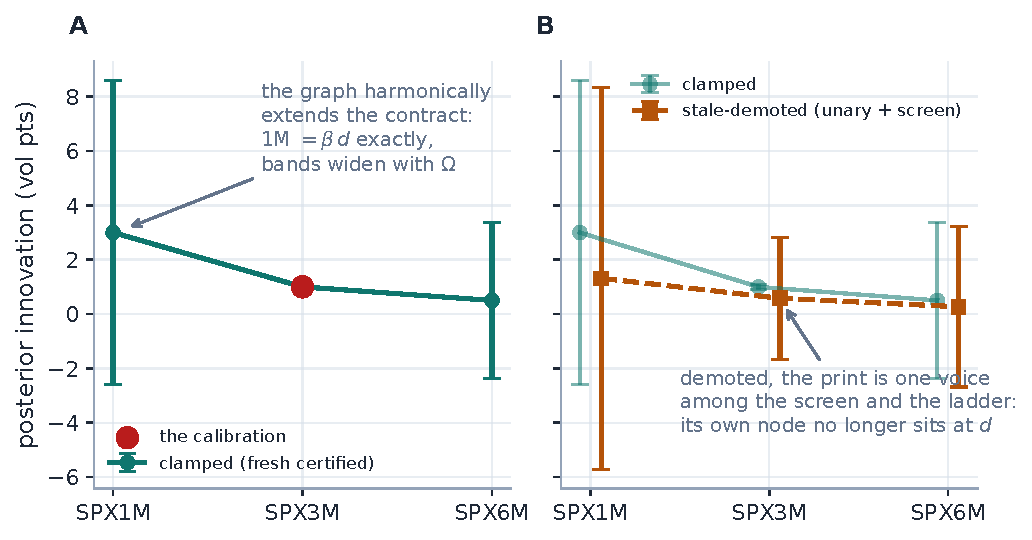
\includegraphics[width=\textwidth]{fig_g3p_boundary.pdf}
\caption{The boundary policy on the SPX ladder (production harmonic
solver, one $+1$ vol-point print at 3M).  A: fresh and certified, the
print is a Dirichlet boundary: its own node publishes $d$ exactly, 1M
lands at the exact contract extension $+\gtpclamponem$, and the boundary's
own calibration uncertainty widens the dependents through $\Omega$.  B:
the same print past the clamp age, demoted to a soft unary anchor under a
screen: its node no longer sits at $d$ (production: $+\gtpsoftthreem$),
the print competes with the ladder and the screen, and every band widens.
Rigidity is earned by freshness and certification --- never granted to a
stale mark.}
\label{fig:boundary}
\end{figure}

\subsection{Who is a boundary: the observation classes}
\label{sec:boundarypolicy}

The workflow sorts every node, at every solve, into one of four classes,
and the sorting is the mode's trading policy.  A \emph{fresh certified}
calibration --- age within the clamp window \emph{and} passing fit
quality, coverage and arbitrage certification; freshness alone is not
sufficient --- is a hard boundary: clamped centrally, uncertainty into
$\Omega$.  A \emph{carried} observation rides its lease as a causal
source state.  A \emph{soft stale} observation is too old to clamp but
not worthless: it demotes to a finite-precision unary anchor and now
\emph{competes} with the parent prediction --- a print from this morning
outvoted, eventually, by what the index has done since
(\cref{fig:boundary}B).  An \emph{unobserved} node receives directed
predictions, harmonic support, its advanced residual, or nothing but the
transported prior.  The four classes are the four possible answers to
``how much should this node's own history bind today's mark?'', and the
dial among them is a stated age policy, not an emergent weight.

\subsection{The decomposition: every mark explains itself}
\label{sec:decomposition}

Because the layers are explicit, every dark mark carries an exact
additive identity --- baseline, plus systematic (what the parents
predict), plus residual (the node's own persisted dislocation), plus
harmonic correction (what reciprocal support added) --- and the wire
reports the four parts with their variances.  \Cref{fig:decomposition}A
shows it through the production pass on the six-node universe of
\cref{sec:universe}: AAPL, carrying a planted $-0.40$-point residual
aged one day under $H=5$, publishes systematic $+\gtpdecompsys$ plus
residual $\gtpdecompres$ $=+\gtpdecomptotal$ vol points, while MSFT ---
same parents, no dislocation --- publishes its systematic alone; the
identity is exact by construction, and panel B sweeps the $\chi$ gauge a
fresh conflicting print would ring.  This is the layered mode's answer to
attribution: not a numerical gain decomposition after the fact, but the
model's own state variables, printed.

\begin{figure}[H]
\centering
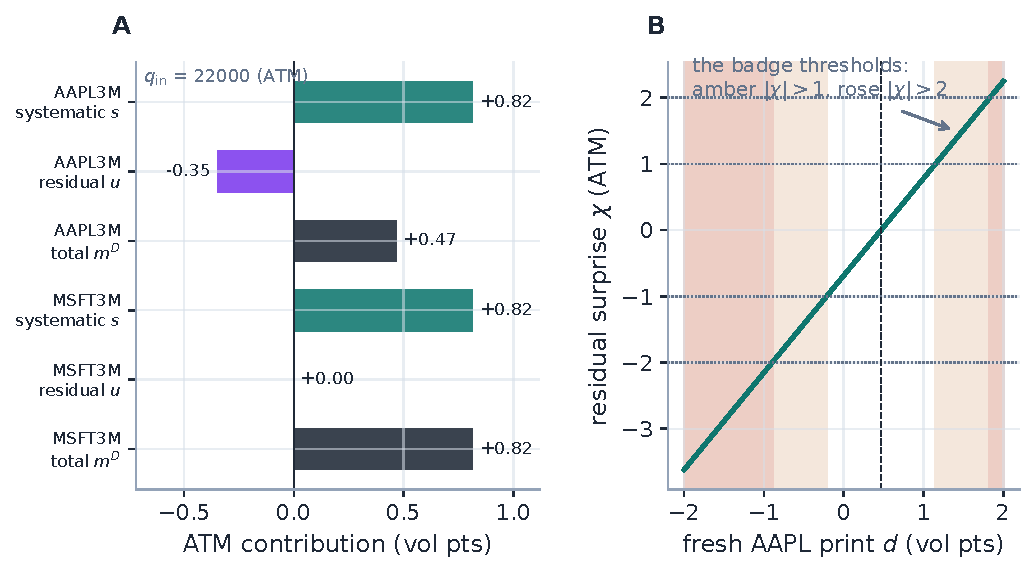
\includegraphics[width=\textwidth]{fig_g3p_decomposition.pdf}
\caption{The mark explains itself (production directed pass, six-node
universe, AAPL carrying a planted $-0.40$-point residual aged one day at
$H=5$).  A: the additive identity per name --- systematic $s$ from the
index and ETF, plus the persisted residual $u$, equals the published
$m^D$; MSFT differs from AAPL exactly by the dislocation.  B: the
residual-surprise gauge \eqref{eq:chi} for a hypothetical fresh AAPL
print: the badge thresholds $|\chi|>1$ (amber) and $|\chi|>2$ (rose) are
the desk's tell for a genuine idio shock versus a bad quote --- the
observation is kept either way; the flag is the product.}
\label{fig:decomposition}
\end{figure}

\begin{figure}[H]
\centering
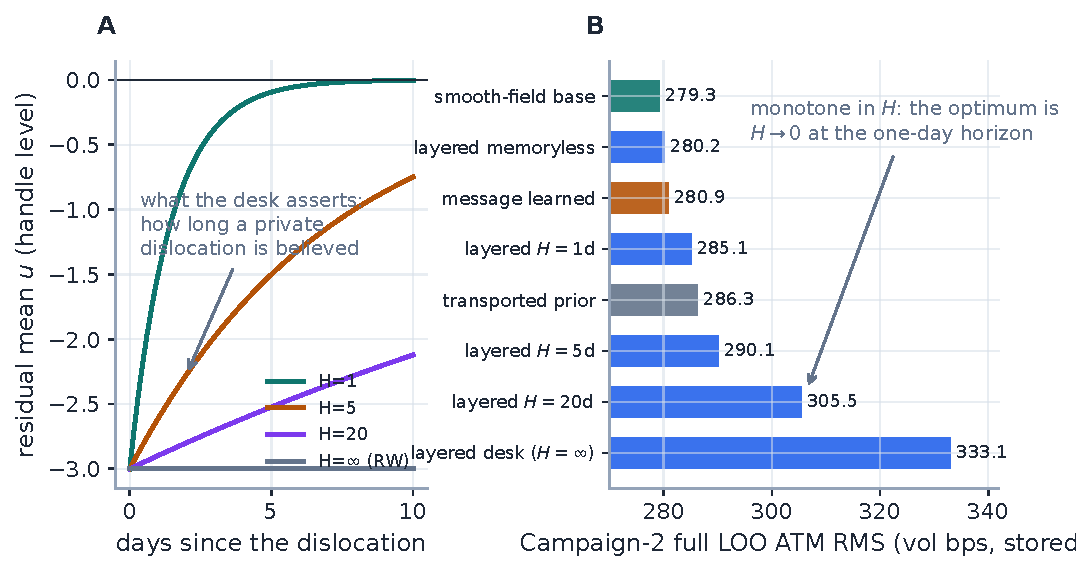
\includegraphics[width=\textwidth]{fig_g3p_halflife.pdf}
\caption{The memory dial, asserted and adjudicated.  A: the production
residual state advancing the story's $\gtpabresidual$-point dislocation
under half-lives $H\in\{1,5,20,\infty\}$ --- the desk's statement of how
long a private dislocation is believed.  B: the recorded Campaign-2
verdict (stored, \cref{sec:evidence}): full-LOO ATM RMS is
\emph{monotone} in $H$ --- memoryless \gtpcampmemoryless\ bps beats
$H{=}1$d (\gtpcamphlone) beats $H{=}5$d (\gtpcamphlfive) beats $H{=}20$d
(\gtpcamphltwenty) beats never-forget (\gtpcampdesk) --- so at the
one-day horizon the optimum is $H\to0$: yesterday's dislocation carries
more noise than signal on this universe.  The assertion the panel-A dial
makes is exactly the one the daily tape declines to reward --- and
exactly the one the intraday experiment must test.}
\label{fig:halflife}
\end{figure}

\subsection{State discipline, and a cautionary case file}
\label{sec:statediscipline}

Persistence buys the desk path; it costs causality discipline, and the
discipline is machinery, not policy prose.  The store threads
chronologically: a residual is advanced \emph{before} any same-time
update; holdout and what-if solves read a pre-dated snapshot and never
write (mutating persistent state would leak the scored day back into
itself); and the store is stamped with a configuration identity ---
change the relations that define a residual's meaning and the affected
entries are purged rather than silently reinterpreted.  Baseline
alignment is part of the same discipline: the residual is defined against
aligned innovations, so a change in the transported baseline between
timestamps must not masquerade as an idiosyncratic move --- if a clean
common-epoch conversion cannot be constructed, the residual takes wider
process variance or is rejected.

\begin{example}[title={Case file: the store that purged itself}]
\textbf{Setup.}  The first adjudication campaign of the layered mode ran
four half-life variants over the frozen benchmark regimes --- and
produced four \emph{byte-identical} result sets, the half-life knob
apparently inert.

\textbf{Diagnosis.}  The benchmark harness re-estimates its cross-relation
betas from each day's data, so they drift daily; the store's
configuration identity hashed the beta \emph{values}; therefore every
day-pair looked like a configuration change and purged the residual
store.  Residuals never survived a single day: the layered mode ran
spatially (its rows differed from the smooth-field arm everywhere) but
with zero temporal memory --- the safety rule, firing on estimation
drift, had silently removed the very thing under test.

\textbf{Fix and lesson.}  The store identity became caller-owned: the
harness pins a stable label per variant, while the structural hash
remains the default so an explicit edit still invalidates --- both
behaviours test-locked.  The invalidated campaign was retained as the
memoryless-layered ablation arm, which is why \cref{fig:halflife}B can
attribute the memory effect specifically.  \emph{A cache-invalidation
rule wired to estimated parameters will fire on estimation noise; state
identity must be owned by whoever defines what ``the same
configuration'' means.}
\end{example}

\paragraph{Exercise 4.}
From \eqref{eq:dynamics} with $H_B$ finite, show that after the $t=3.5$
update of \cref{sec:story} the $t=4$ mark is
$14-3\cdot2^{-0.5/H_B}\ge11$, with equality as $H_B\to\infty$: mean
reversion can only make $B$ catch \emph{up} to $A$ faster --- no
half-life explains a mark below $11$, which is why the flat staircase
identifies a long half-life and why ``forget faster'' is the only
memory dial the data of \cref{fig:halflife}B could ask for.

%======================================================================
\section{One universe, three answers}
\label{sec:universe}

The three assertions are now side by side on one miniature universe ---
an SPX calendar ladder (1M/3M/6M), the sector ETF XLK, two technology
names; lit: SPX~3M $+1.00$ vol point and XLK~3M $+0.55$
(\cref{fig:spectrum}).  Every difference in the figure is an assertion,
not a tuning.  At SPX~1M the layered mode publishes $+\gtpspeclayonem$
--- the full $\alpha_T{=}1$ contract through the clamped boundary; the
learned message level publishes $+\gtpspecmsgonem$ --- the same contract
shrunk by the measured calendar transfer; the smooth field publishes
$+\gtpspecsmoothonem$ --- not a contract at all, but the smoothness
compromise between the lit move and the zero anchor.  At the dark names
the message and layered answers nearly agree (corroborated index-and-ETF
transfer) while the smooth field hears the same signals as generic
neighbour pressure.  None of the three is ``the wrong number'' --- each
is the exact consequence of its prior, which is the note's thesis in one
picture.  But put a trader in front of the figure and ask which column
they would initial: only the layered column is, number by number, the
direct consequence of sentences the desk actually said --- the other two
are what a solver concludes when the desk says less.

\begin{figure}[H]
\centering
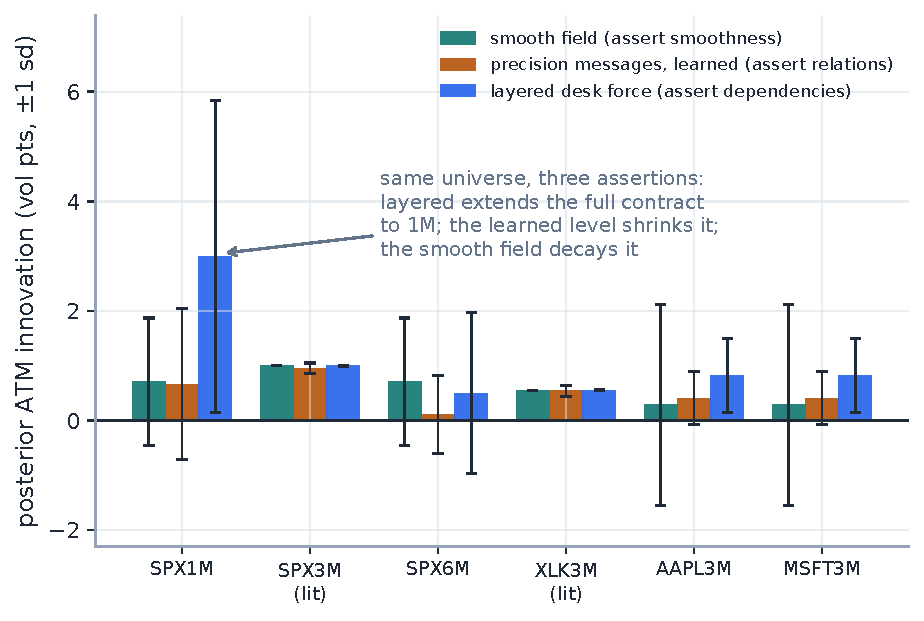
\includegraphics[width=0.98\textwidth]{fig_g3p_spectrum.pdf}
\caption{The thesis figure: one universe (SPX ladder + XLK + two names,
two lit calibrations), three production solves.  Layered desk force
extends the full calendar contract to 1M ($+\gtpspeclayonem$); the
learned message level shrinks the same contract to $+\gtpspecmsgonem$;
the smooth field, asserting no contract, decays the move to
$+\gtpspecsmoothonem$.  At the dark names the two contract modes agree
(corroborated cross transfer) while the smooth field treats the signals
as neighbour pressure.  Bars carry $\pm1$ posterior sd: the layered 1M
band is the boundary's $\Omega$-widened uncertainty, not false
confidence.}
\label{fig:spectrum}
\end{figure}

\subsection{The desk surface}
\label{sec:surface}

The mode dial and every object in this note are first-class in the
product's Graph workspace, and four screenshots close the loop from
mathematics to desk.  \Cref{fig:shotshell} is the shell after a layered
what-if run: a $+1$ vol-point pulse on SPY's 18-month node spreads through
its own calendar ladder and across the cross relations to QQQ and AAPL;
the top bar carries the observation-source toggle, the three-mode
propagation segment with \textsf{Layered} active, the configuration and
preflight chips, and the run summary (1 observed, 11 extrapolated); the
canvas colours posterior shift and rings observed nodes; the diagnostics
drawer is already raising the loud-$\chi$ banner of \eqref{eq:chi}.
\Cref{fig:shotpanes} shows the two configuration surfaces: the
relationships pane (left) states the calendar policy in desk units ---
amplitude preset, level $\rho$, shape $\alpha_T$, decay family and its
$\epsilon_T$, with a live worked example (``6M informs 3M: $+1.00$ pt
$\to$ $+2.00$ pt message, relationship uncertainty $2.94$ pt'') --- and
the per-relation editor (right) lists every relation with its class, its
\emph{semantics} column (auto $\cdot$ reciprocal versus directed --- the
\cref{sec:layered} split, per row), its precision-rule chip, per-handle
betas and the implied-reverse reading of \cref{sec:rowform}, above a
scenario preview locked to this note's golden numbers.
\Cref{fig:shotinspector} is the inspector on a dark AAPL node after the
layered run: the decomposition card prints the \cref{sec:decomposition}
identity (baseline $20.0\%$, systematic $+0.0$, residual $+0.0$, harmonic
$+71.6$ bp --- the auto taxonomy is all-reciprocal, so the move rides the
harmonic layer), the incoming-messages table lists each relation's
$z\cdot\beta$ message with the $\Leftarrow$ implied-reverse row, and the
footer states Exercise~3's lesson verbatim: local consensus $+72.1$ bp at
conditional confidence $q$, final marginal $+71.6\pm118$ bp --- ``local
$\neq$ final: the marginal folds in informer uncertainty and shared-route
covariance --- trust the final.''

\begin{figure}[H]
\centering
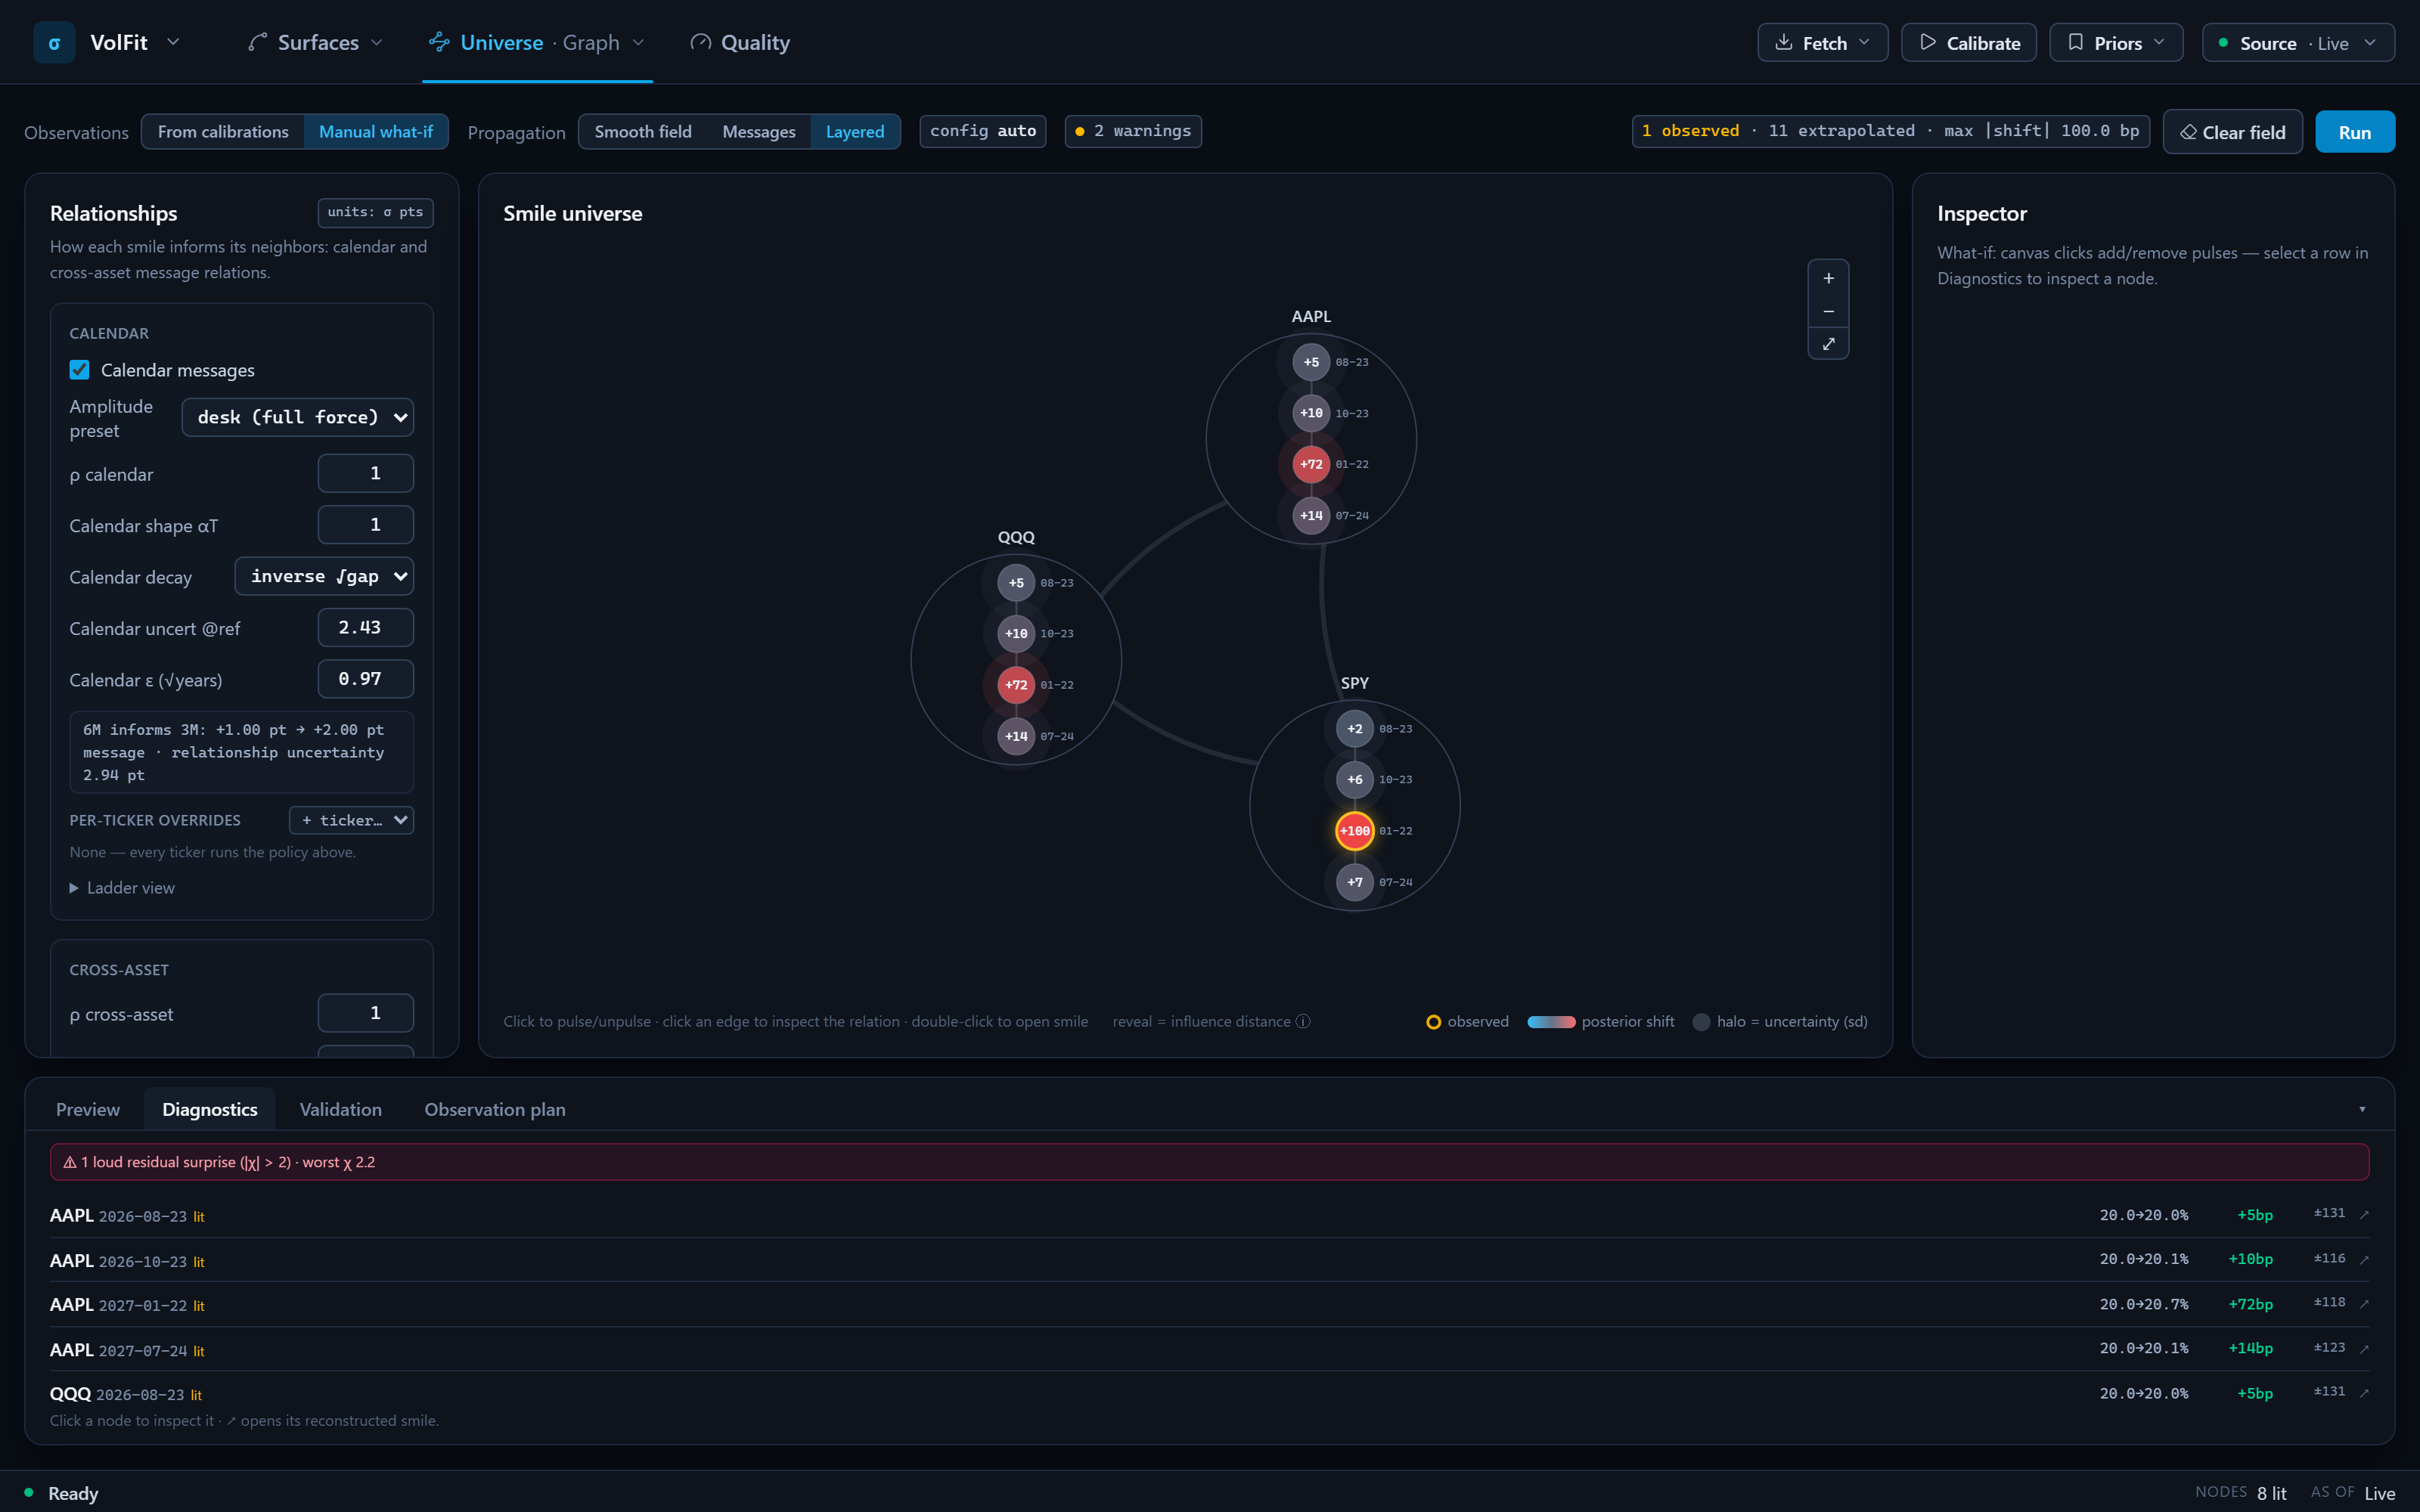
\includegraphics[width=\textwidth]{shot_g3p_shell.png}
\caption{The Graph workspace after a layered what-if run (live capture).
Top bar: observation source, the three-mode segment (\textsf{Layered}
active), config and preflight chips, run summary.  Canvas: the $+1$
vol-point pulse on SPY 18M spreading through the calendar ladder and the
cross relations; observed nodes ringed, posterior shift coloured.
Drawer: the diagnostics table with the loud-$\chi$ residual-surprise
banner.}
\label{fig:shotshell}
\end{figure}

\begin{figure}[H]
\centering
\begin{minipage}[t]{0.315\textwidth}
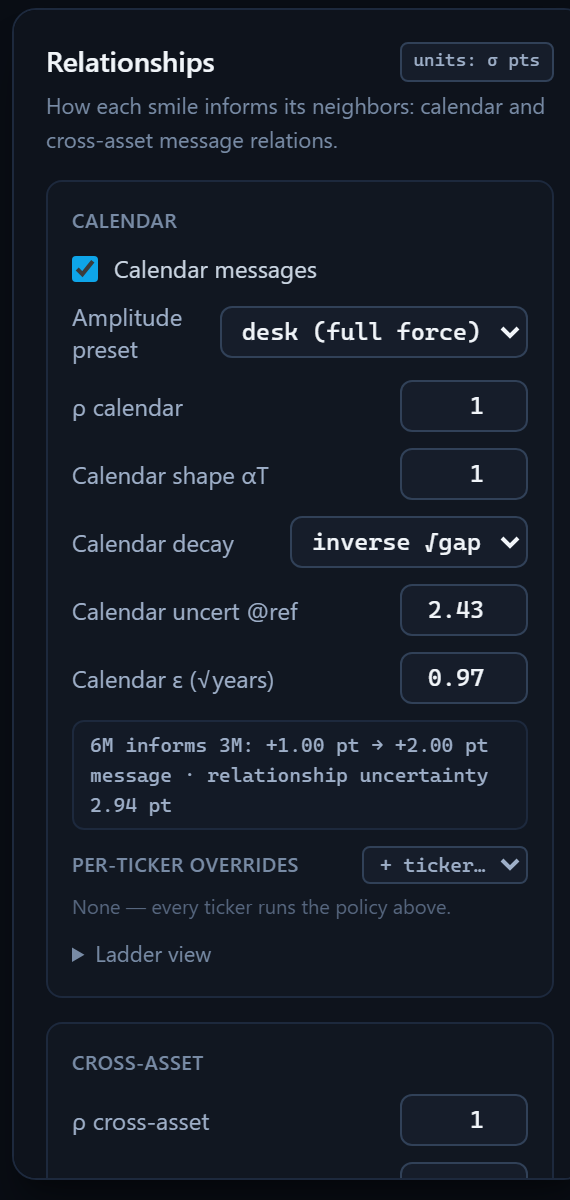
\includegraphics[width=\textwidth]{shot_g3p_policy.png}
\end{minipage}\hfill
\begin{minipage}[t]{0.655\textwidth}
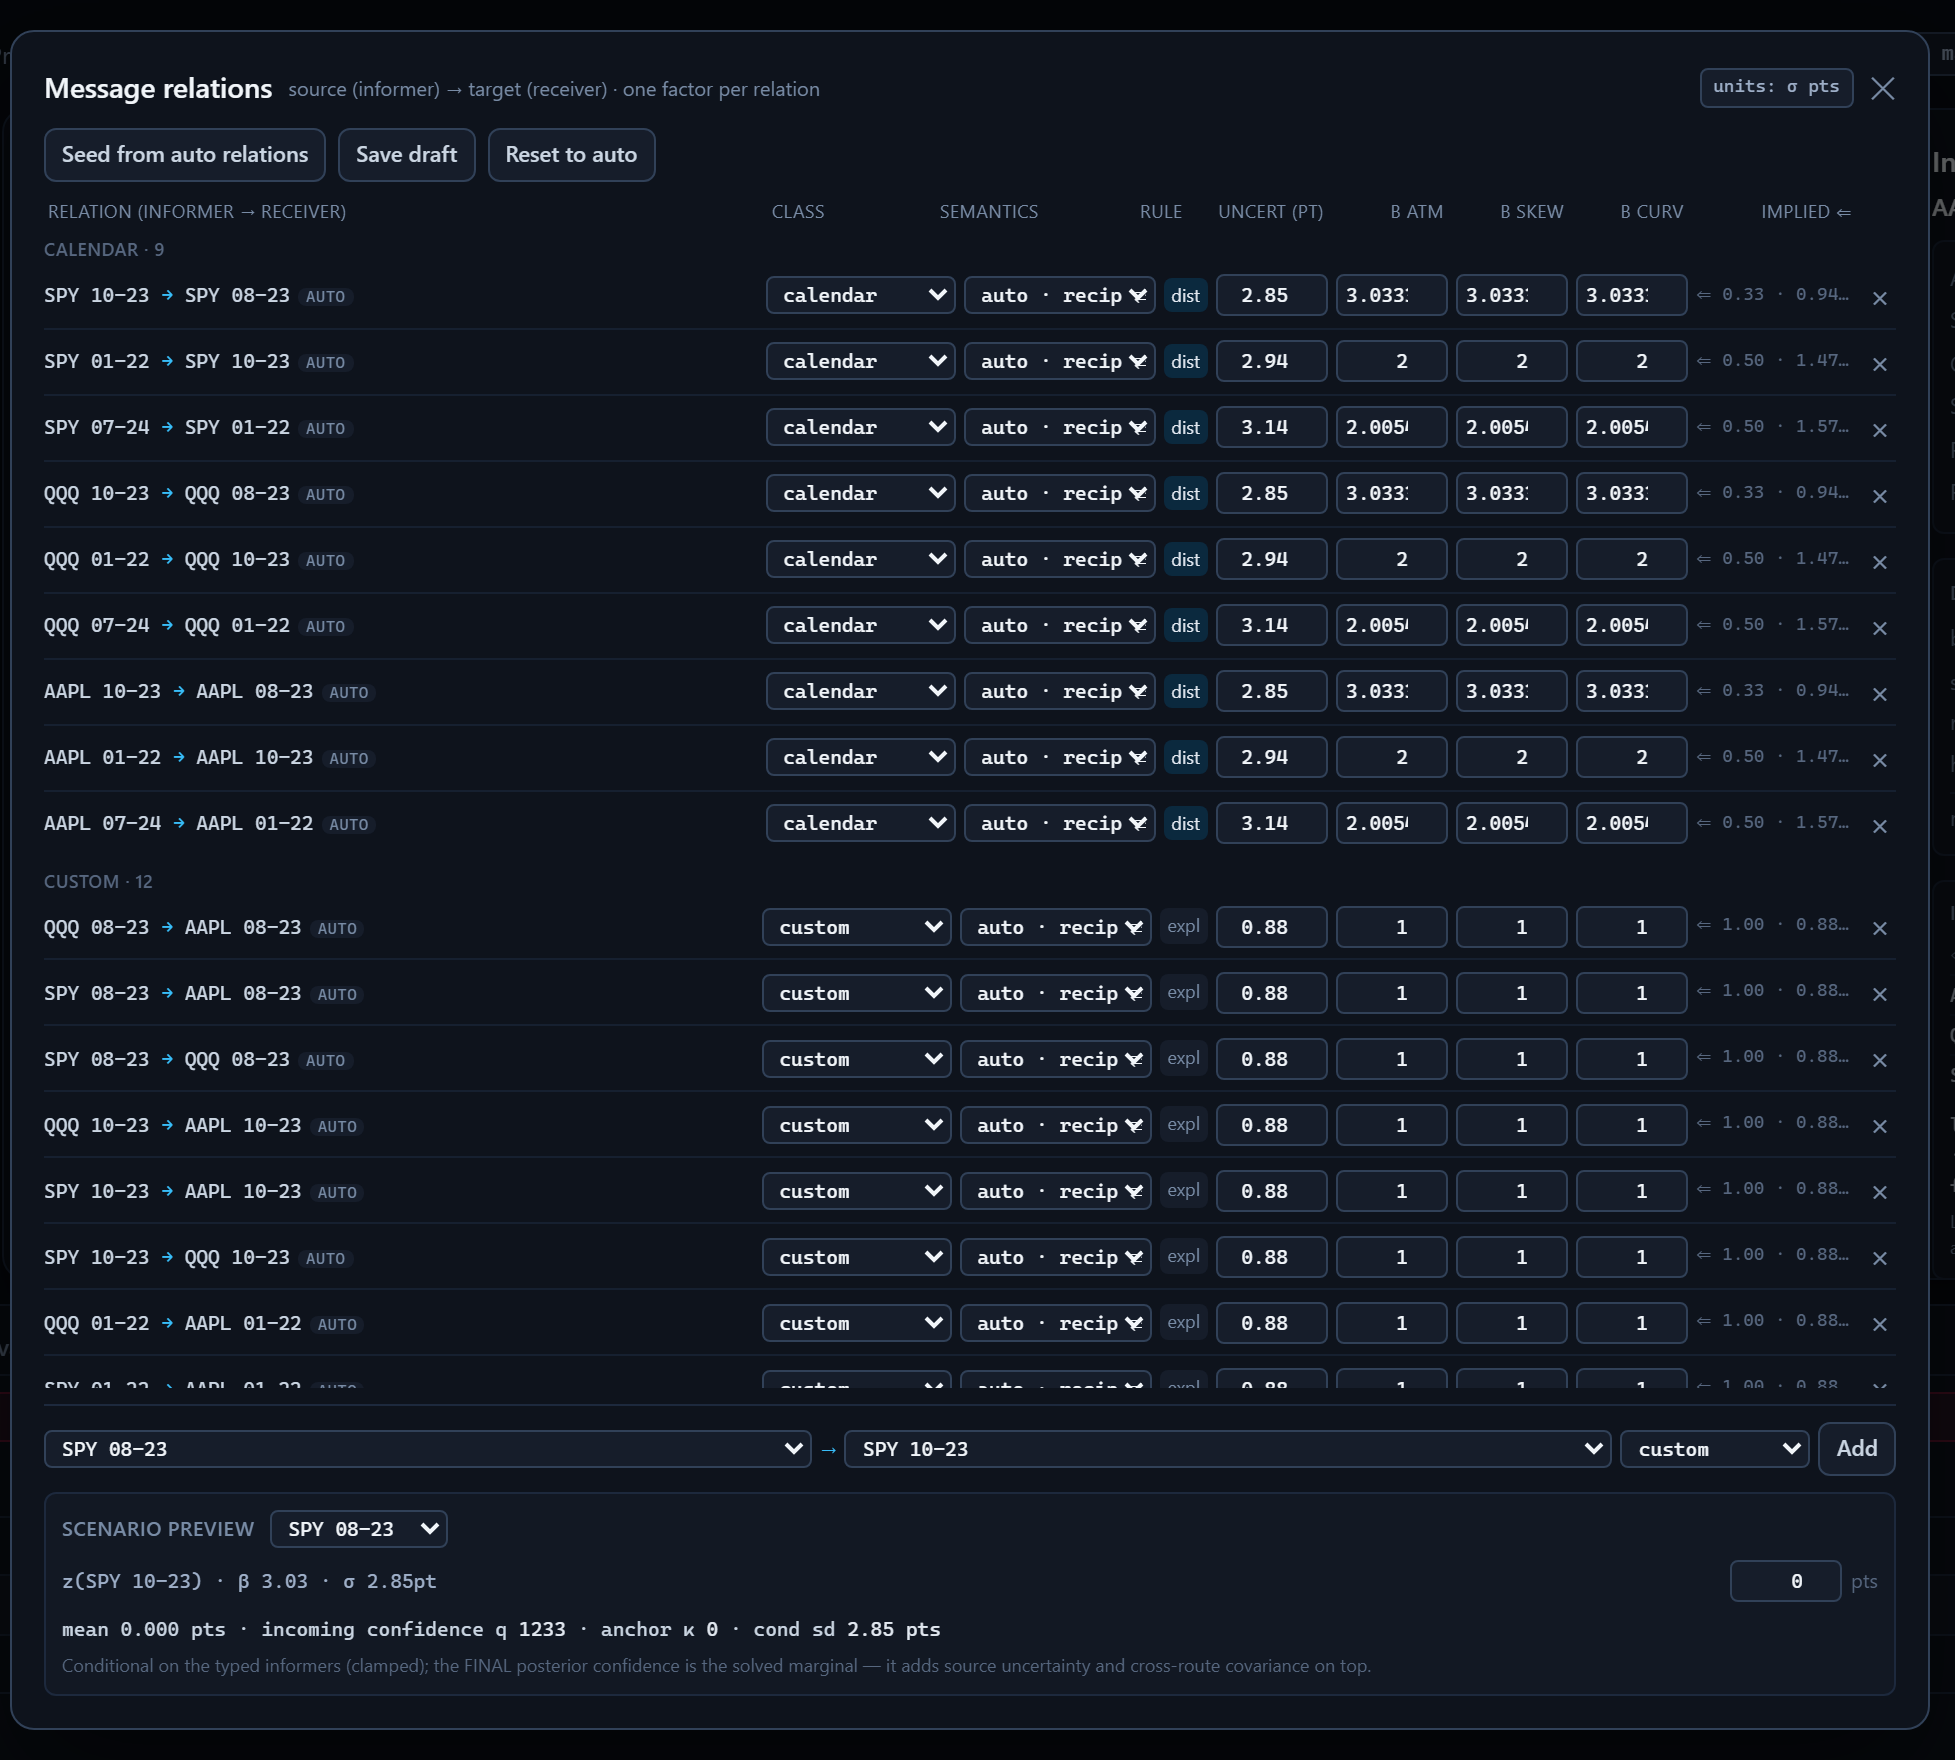
\includegraphics[width=\textwidth]{shot_g3p_editor.png}
\end{minipage}
\caption{Configuration in desk units (live captures).  Left: the
calendar policy card --- amplitude preset and level $\rho$, shape
$\alpha_T$, decay family with $\epsilon_T$, and a live worked example of
the \cref{sec:messages} contract.  Right: the per-relation editor ---
class, the per-row \emph{semantics} column (reciprocal vs directed, the
\cref{sec:layered} split), precision rule, per-handle betas, and the
implied-reverse column of the canonical-orientation identity; the
scenario preview at the bottom is locked to this note's golden numbers.}
\label{fig:shotpanes}
\end{figure}

\begin{figure}[H]
\centering
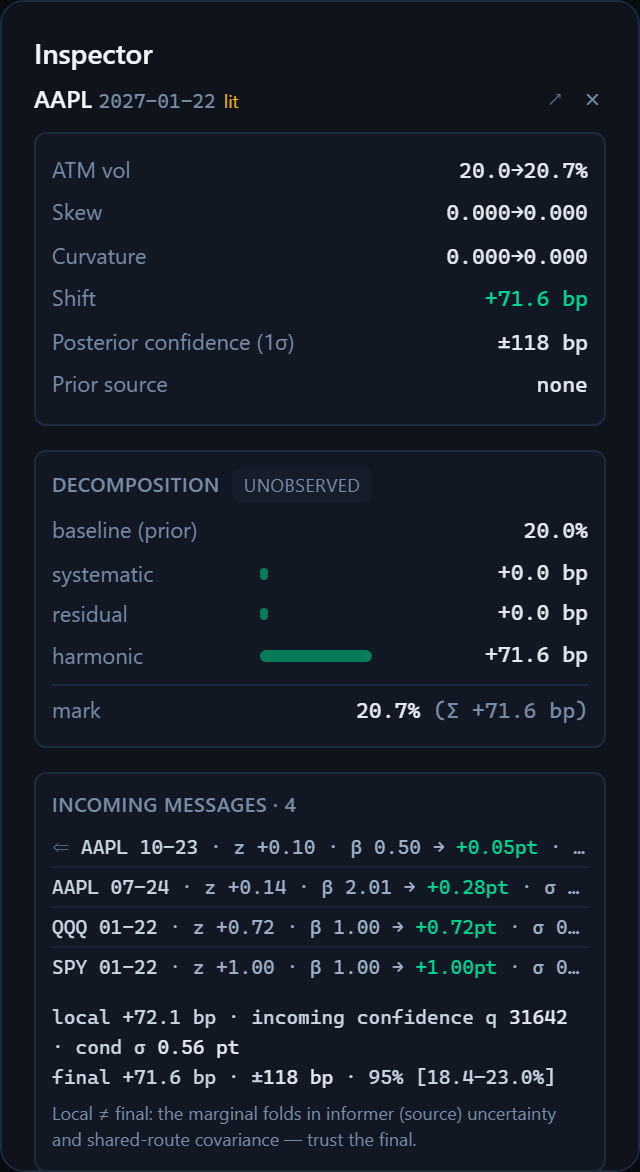
\includegraphics[width=0.42\textwidth]{shot_g3p_inspector.png}
\caption{The inspector on a dark name after a layered run (live
capture): the decomposition identity of \cref{sec:decomposition} as a
card (this auto-taxonomy run is all-reciprocal, so the move rides the
harmonic part), the incoming messages with the implied-reverse row, and
the local-vs-final distinction of Exercise~3 stated as product copy.}
\label{fig:shotinspector}
\end{figure}

%======================================================================
\section{Evidence and the gates}
\label{sec:evidence}

The empirical discipline runs in three layers, and this section quotes
its records --- including the ones that decline to flatter the note's
most expressive mode.

\textbf{Golden contracts.}  Every mean-semantics behaviour of
\cref{sec:messages,sec:layered} --- full transmission, competition,
cross-asset averaging, multi-hop accumulation, the dead informer, the
repeated path, shrunk-mode corroboration, baseline-once, the
asynchronous A/B path, zero reverse influence, exact target ownership,
store invalidation --- is a fixture with an expected number, checked
against an independent brute-force Gaussian reference and reproduced
through the production modules at $10^{-12}$ (the A/B staircase of
\cref{fig:asyncab}A is replayed against the golden fixture inside this
note's own figure generator).  The smooth field is locked differently
but equally: byte-identity of the shipped default against the full
legacy suite.

\textbf{The design study.}  The empirical levels quoted throughout ---
transfer slopes \gtprhoindex\ (index), \gtprhopeer\ (peer),
\gtpcallevel\ (calendar), the corroboration adjudication of
\cref{fig:amplitude}, the calendar noise seeds of \cref{fig:calendar}
--- come from a stored study over three historical regimes of benchmark
rows, read from its artifact, never re-run.  The same row bank measured
the spine's extrapolation skill (the smooth-field record of
\cref{sec:smooth}), so graph extrapolation as such is not the hypothesis
under test in what follows; the marginal value of each \emph{assertion}
is.

\textbf{Gate one: do contracts beat smoothness?}  The message mode's
promotion to default was pre-registered: material dark-name skill over
both the transported prior and the smooth field, no stressed-regime
degradation, no calm harm beyond tolerance, honest bands
($\operatorname{std}\zeta\approx1$, coverage near nominal), no unstable
cycles, no wing deterioration --- with the recorded expectation that the
\texttt{desk} preset would lose day-horizon RMS (it is a belief mode and
ships regardless; the gate adjudicates the \emph{default}).  The
campaign's intersected verdict: message-learned full-LOO ATM RMS
\gtpcampmsg\ bps against the smooth-field base \gtpcampbase\ --- no
material edge, bands running narrow
($\operatorname{std}\zeta\ \gtpzetamsg$ against the base's over-wide
\gtpzetabase) --- so \emph{no default change}: the contract mode ships as
an explicit switch, its semantics the reason to choose it, not its RMS.

\textbf{Gate two: does the layered assertion pay?}  The layered mode's
pre-registered table was adjudicated on \gtpcamppairs\ intersected
out-of-sample rows across seven arms, and the verdict is the most
instructive record in the project: \emph{record, hold adoption}.  Three
findings, stated exactly --- and in the order a desk should read them.
(i) \emph{The layered spatial solve carries the family's only measured
edge in the stressed regimes}: against the smooth-field base, warm
full-LOO improves by \gtpstressspike\ bps in the August-2024 spike and
\gtpstresshigh\ in the October-2022 bear --- the two regimes where books
actually bleed and where every other arm, message mode included, adds
nothing.  The directed clamp-and-cut helps exactly when systematic moves
dominate, which is the mechanism doing what it was designed to do; the
price is \gtpcalmcost\ bps in the calm regime, when there is little
systematic signal for the structure to carry.  (ii) \emph{Day-old
residual memory does not pay}: full-LOO RMS is monotone in the half-life
(\cref{fig:halflife}B) --- the memoryless layered arm
(\gtpcampmemoryless) beats every finite $H$ and the never-forget desk arm
(\gtpcampdesk) --- so at daily granularity the optimum is $H\to0$:
yesterday's private dislocation is noise by the next morning.  Note the
scope of that sentence before generalizing it: the harness can only test
dislocations that are a full day old, and \cref{sec:story}'s dislocation
was hours old --- the finding prices one dial (memory) at one horizon
(daily) on one universe; it does not price the mode, whose spatial half
just posted the edge in (i) \emph{with the memory switched off}.
(iii) \emph{Calibration and wings flag real work}:
$\operatorname{std}\zeta\ \gtpzetahl$ (the diagonal unary anchors
understate dark-node variance when predictions share parents --- the
joint block is wired and first in line), and a wing-RMS regression
(\gtpwingliquid\ vs \gtpwingliquidtransport\ bps on the liquid split)
traced to the harness broadcasting vol-normalized ATM betas to the shape
handles --- partially mitigated since, with full-amplitude shape transfer
through directed anchors still an open pass.  The decision:
\texttt{smooth\_field} remains the default; the layered mode is a
session-level opt-in --- deliberately never seeded from saved options ---
and the message-gate verdict stands unchanged.

\textbf{The honest scope caveat, and the decisive experiment.}  The
campaign tests \emph{daily} granularity, where every held-out node
relights every day.  The layered mode's target regime --- the
\cref{sec:story} story: a name lit once mid-session, marked against a
moving liquid source, dislocations living for hours --- is precisely what
a daily harness cannot see; the one arena the mode was built for has not
yet been scored.  At day granularity the recorded answer is ``don't carry
the state''; whether the assertion pays \emph{intraday} is the
pre-registered asynchronous timestamp replay over stored tick-history,
and this note --- like its predecessor with the message gate --- refuses
to pre-empt a verdict that is not in.  But the reader should be clear
about what does \emph{not} wait on that experiment.  Direction, rigidity
and the decomposition are not hypotheses under test --- they are audit
requirements, and no RMS result can substitute for them: a solver that
lets a satellite print mark down the index is not a slightly less
accurate solver, it is a wrong one, whatever its score.  On those
requirements the layered mode is not the leading candidate --- it is the
only candidate; the open experiment decides how hard to lean on its
memory, not whether the desk needs its language.

%======================================================================
\section{What is genuinely original here}
\label{sec:original}

Gaussian fields, factor graphs and state-space models are classical; the
synthesis is specific.  \emph{The assertion dial as an architecture}:
three priors of strictly increasing structure behind one seam, so the
desk chooses what to claim, not which product to buy --- and the modes
are honest about being different questions, not rival answers to one.
\emph{Contractual propagation for volatility}: every desk-facing
behaviour a golden-locked theorem, amplitude split into locked shape and
measured level, the level mechanized by a node-linked anchor validated on
stored rows to \gtppredgap\% with zero free parameters.  \emph{The
dead-informer analysis}: a joint-distribution defect invisible to every
local conditional, surfaced and used to select the factor form.  \emph{A
trading-native state layer}: influence arcs cut at the source, residual
memory with an asserted half-life, boundary rigidity earned by
certification --- with the causal replay itself a golden acceptance test.
\emph{Honesty rules as first-class machinery}: improper components left
improper, baseline uncertainty placed exactly once, attribution by
source, marks that print their own decomposition.  And \emph{evidence
discipline}: pre-registered gates, expectations recorded before sweeps,
negative findings (memory at the day horizon; the message RMS tie)
published in the same breath as the wins --- with the store-purge case
file kept as a lesson rather than buried.

%======================================================================
\section{Limitations}
\label{sec:limits}

Where the guarantees stop, per mode and shared.  \emph{The layered
adjudication is scoped}: its recorded verdict is daily-granularity; the
intraday replay --- the regime the mode was designed for --- is open, and
until it lands the mode's aggregate day-horizon RMS is not its selling
point (its stressed-regime edge and its semantics already are; both are
on the record above).  \emph{Correlated informers and parents}: the message $q_i$ adds
configured precisions as if conditionally independent, and the layered
v1 unary anchors are diagonal --- both overstate joint confidence when
sources share a factor (the recorded
$\operatorname{std}\zeta\ \gtpzetahl$); the exact joint block exists in
the solver and its adjudication is first in line.  \emph{Shape transfer
through directed anchors is unfinished}: broadcasting vol-normalized ATM
amplitudes to skew and curvature caused the recorded wing regression;
the harness now pins unit shape betas, and a measured shape amplitude
(or zero cross shape transfer) is an open pass.  \emph{Cross-class
precision seeds are upper bounds} (ticker-median measurement).  \emph{The
amplitude shape is weakly identified at the day horizon} --- $\alpha_T=1$
is held by semantics, not by $R^2$.  \emph{Hybrid mode is machinery, not
a recommendation} (validated only at its zero-weight identity with pure
messages).  \emph{The solves are dense}, sized for the
$O(10^2$--$10^3)$-node selected universe; the factor lists and the DAG
pass are sparse-ready.  \emph{Residual state requires common-epoch
alignment}: baseline transport between timestamps can masquerade as an
idiosyncratic move, and the discipline is wider variance or rejection,
never silent trust.  \emph{Calendar arbitrage remains soft} in all three
modes: propagation moves maturity signals but imposes no hard
cross-expiry projection --- publish-time diagnostics and the projection
of Note~09 remain the fence.  And \emph{curvature stays the weakest
handle} end to end, in identification and in units.

\appendix
%======================================================================
\section{Hyperparameter atlas}
\label{app:atlas}

The only home for settings names: the body speaks mathematics, this table
speaks configuration.

\begingroup
\small
\begin{longtable}{p{0.34\textwidth}p{0.15\textwidth}p{0.43\textwidth}}
\caption{Propagation-mode hyperparameters.}\label{tab:atlas}\\
\toprule Knob & Default & Role\\ \midrule
\endfirsthead \toprule Knob & Default & Role\\ \midrule \endhead
\texttt{propagationMode} & \texttt{smooth\_field} & The dial:
\texttt{smooth\_field} / \texttt{precision\_messages} / \texttt{hybrid}
(config-only) / \texttt{layered\_dynamic\_harmonic}.  The default is
gate-adjudicated (\cref{sec:evidence}); the layered value is a
session-level opt-in --- saved options never seed it.\\
\midrule
\multicolumn{3}{l}{\emph{Smooth field (\cref{sec:smooth})}}\\ \midrule
$\eta$, $\kappa$ & autotuned & Directed-smoothness weight (reach);
local-smallness anchor.  Seeded from saved options; marginal-likelihood
autotune available.\\
$\lambda$, $\nu$ & $0$, $0.1$ & Optimal-transport tangent term (off by
default) and its source allowance.\\
edge weights / $\beta$ overrides & auto-lattice & Raw trust weights and
per-edge amplitude overrides on the calendar/cross lattice.\\
\midrule
\multicolumn{3}{l}{\emph{Messages (\cref{sec:messages})}}\\ \midrule
\texttt{calendarBetaExponent} & $1.0$ (per handle) & The amplitude shape
$\alpha_T$ of \eqref{eq:beta}.\\
\texttt{calendarAmplitude} / \texttt{crossAmplitude} & $1.0$ & Class
levels $\rho$; presets desk $=1.0$ / learned $\approx0.23$ calendar,
$\approx0.39$ index ($\alpha_T{=}1$ values).\\
\texttt{calendarPrecisionScale} $p_0$, \texttt{Epsilon} $\epsilon_T$,
\texttt{Decay} & $1.7{\times}10^3$, $0.97$, inv-$\sqrt{\text{gap}}$ &
The confidence family \eqref{eq:calprec}; constant and log-distance
ablations ship beside it.\\
\texttt{crossPrecisionScale} & $1.3\times10^4$ & Constant cross-relation
precision (index seed; upper bound).\\
\texttt{innovationAnchorPrecision} & derived & Override for
\eqref{eq:anchor}; unset $=$ node-linked from $\rho$; $\rho=1$ gives
$\kappa=0$ exactly.\\
\texttt{cycleBetaTolerance} & $10^{-9}$ & Gauge-sweep flag threshold.\\
\texttt{messageEdges} / persisted rules & --- & Request relations $\to$
persisted schema rules $\to$ auto relations, in that precedence; draft
and active configurations are versioned with an event log.\\
\midrule
\multicolumn{3}{l}{\emph{Layered (\cref{sec:layered})}}\\ \midrule
\texttt{relationSemantics} & class default & Per-row
\texttt{reciprocal\_harmonic} / \texttt{directed\_state}; defaults:
calendar, sector peer, custom $\to$ reciprocal; broad index, sector ETF
$\to$ directed.  Auto relations are always reciprocal --- a directed arc
is an explicit configuration.  Directed cycles are rejected.\\
\texttt{clampMaxAgeDays} & $1$ & The freshness window for hard Dirichlet
boundaries; older certified observations demote to soft unary anchors
(\cref{sec:boundarypolicy}).\\
\texttt{residualHalfLife} & never (RW) & The memory dial $H$ of
\eqref{eq:dynamics}; per-handle broadcastable.\\
\texttt{residualConfigVersion} & structural hash & The store identity:
caller-owned stable label, else a structural hash of the relations ---
changed identity purges affected residuals
(\cref{sec:statediscipline}).\\
residual store & persisted & Restored at startup, written only by real
layered solves on certified target observations; what-if and holdout
solves never write.\\
screen $\kappa$ & $0$ & Screened-harmonic retention toward the prior
(\cref{sec:harmonic}); $\kappa>0$ is a stated policy, not an extension.\\
\midrule
\multicolumn{3}{l}{\emph{Hidden (module constants)}}\\ \midrule
\texttt{HANDLE\_PRECISION\_SCALE} & $(1,0.36,0.0036)$ & Per-handle
precision units (\cref{sec:amplitude}).\\
\texttt{RELATION\_CLASSES} & 5 classes & calendar / broad\_index /
sector\_etf / sector\_peer / custom.\\
\texttt{DISCONNECTED\_Z\_SD} & $(0.03,0.05,0.5)$ & The honest
no-active-path innovation sd per handle (one typical move).\\
canonical orientation & shorter $T$ & Auto calendar receiver; reverse
identity $p_{j\leftarrow i}=p_{i\leftarrow j}\beta^2$.\\
\bottomrule
\end{longtable}
\endgroup

%======================================================================
\section{Performance notes}
\label{app:perf}

\begin{enumerate}[leftmargin=1.6em]
\item \textbf{All three solves are dense at the current design point}
($O(10^2$--$10^3)$ nodes) and sparse-ready beyond it: the message factor
list is $O(E)$ triplets with no normalization coupling; the layered
directed pass is $O(E_D)$ per handle in topological order; the harmonic
completion inverts per factor-support component, so one disconnected
block never pays for another and the Cholesky guard localizes any
conditioning failure to a named component.
\item \textbf{The smooth field solves in covariance form} because
$n_{\mathrm{obs}}\ll N$: only the observed columns and one
$m\times m$ solve, marginals by a single contraction --- no dense
posterior matrix is formed; the same stored columns price the
observation-selection question (which dark node is worth quoting next)
in closed form.
\item \textbf{The mode fork adds no data work}: universe, transported
priors, innovations and calibration precisions are computed once,
upstream of the fork; the layered mode adds only the residual-store
read/advance and its persistence write-back.
\item \textbf{Adjudication runs where long jobs survive}: the campaigns
execute from the user's own shell (chunked, resumable parts beside the
frozen fixtures); tool-spawned background jobs are killed on this box ---
a recorded operational constraint.
\item No benchmark in this note was re-timed; figures and golden numbers
were generated at commit \texttt{\gtpgencommit} on \gtpgendate\ through
the production modules, and every campaign or design-study number is
read from its stored artifact.
\end{enumerate}

%======================================================================
\section{Traceability}
\label{app:trace}

\begingroup
\small
\setlength{\tabcolsep}{3pt}
\begin{longtable}{@{}p{0.34\textwidth}p{0.14\textwidth}p{0.25\textwidth}p{0.22\textwidth}@{}}
\caption{Claims in this note and the code/tests that lock them.}\\
\toprule Claim & Object & Code anchor & Test anchor\\ \midrule
\endfirsthead
\toprule Claim & Object & Code anchor & Test anchor\\ \midrule
\endhead
Smooth-field prior, kernel/stationary mass, covariance update, marginal
honesty, byte-locked default &
\eqref{eq:qsm}, \cref{sec:smooth} &
\nolinkurl{volfit/graph/\{build,operators,prior,posterior\}.py} &
\nolinkurl{test_graph_example.py}, legacy suite byte-identity\\
Pairwise operator PSD; receiver conditional; canonical orientation;
$q_i$ unit mapping &
\eqref{eq:qmsg}, \cref{prop:conditional} &
\nolinkurl{volfit/graph/message.py} &
\nolinkurl{test_graph_message.py}\\
Golden message contracts (transmission, competition, multi-hop, dead
informer, repeated path, corroboration, baseline-once) &
\cref{sec:messages} &
\nolinkurl{tests/fixtures/graph_message_golden.json} &
\nolinkurl{test_graph_message_golden.py} (brute-force reference)\\
Information-form component solve; no-lit honesty; reachability guard;
exact attribution &
\eqref{eq:posterior} &
\nolinkurl{volfit/graph/message_posterior.py} &
\nolinkurl{test_graph_message_posterior.py}\\
Residual state, dynamics, leases, hard/Kalman updates, causal ordering,
store round-trips &
\cref{sec:state} &
\nolinkurl{volfit/graph/temporal_state.py} &
\nolinkurl{test_graph_temporal_state.py} (A/B exit gate)\\
Directed pass: exact parent covariance, cut at source, DAG rejection,
attribution, $\chi$ &
\eqref{eq:directedpred}--\eqref{eq:chi} &
\nolinkurl{volfit/graph/directed_state.py} &
\nolinkurl{test_graph_directed_state.py}\\
Harmonic completion: Dirichlet partition, $\Omega$, unary anchors
(diag + joint), screen, gauge strictness &
\eqref{eq:dirichlet} &
\nolinkurl{volfit/graph/harmonic_posterior.py} &
\nolinkurl{test_graph_harmonic_posterior.py}\\
Layered orchestration: semantics defaults, boundary policy, store
persistence + invalidation, what-if/holdout read-only &
\cref{sec:boundarypolicy,sec:statediscipline} &
\nolinkurl{volfit/api/graph_dynamic.py} &
\nolinkurl{test_graph_dynamic_production.py},
\nolinkurl{test_graph_dynamic_golden.py}\\
Mode fork, auto relations, $r^d$ harmonic, band placement, hybrid
zero-weight identity, editor/scenario preview locks &
\cref{sec:universe} &
\nolinkurl{volfit/api/graph_message.py},
\nolinkurl{api/graph_extrapolation.py} &
\nolinkurl{test_graph_message_production.py}, frontend vitest locks\\
Campaign records (message gate; layered §16.3 table; store-purge post
mortem) &
\cref{sec:evidence} &
\nolinkurl{backtest/FINDINGS_message_phase4.md},
\nolinkurl{backtest/FINDINGS_dynamic_phase5.md} &
stored parts under \nolinkurl{backtest/results/benchmark/}\\
Design study (anchor choice, seeds, learned levels) &
\cref{sec:amplitude} &
\nolinkurl{backtest/message_phase0.py} &
artifact \nolinkurl{results/message_phase0.json} (regenerable)\\
\bottomrule
\end{longtable}
\endgroup

%======================================================================
\section{Reference implementation}
\label{app:ref}

Each mode's core is a few lines, executed against the production modules
before this note was built.  The message listing (operator, anchors,
information-form solve) agrees with production to \gtprefagreemsg\ on a
four-node directed universe, and the gauge sweep cross-check flags
nothing on a consistent triangle (\gtpcycleflags\ flags) while reporting
the planted inconsistent product \gtpcyclebad.  The layered listing
(directed means and variances by hand on a three-node chain, plus the
Dirichlet extension $-Q_{H,FF}^{-1}Q_{H,FS}d_S$ assembled from raw
factors) agrees to \gtprefagreelay.  The smooth listing (stationary mass
and the $\beta$-weighted directed residual) agrees to \gtprefagreesm.

\begin{lstlisting}[caption={The three cores (verified against
\texttt{volfit.graph}; agreements stated above).}]
def message_operator(n, factors):        # factors: (i, j, p, beta)
    Q = np.zeros((n, n))
    for i, j, p, b in factors:
        u = np.zeros(n); u[i] = 1.0; u[j] = -b
        Q += p * np.outer(u, u)          # PSD for any real beta
    return Q                             # posterior: Q + diag(kappa) + H^T R H

def directed_predict(parents, p, beta, m_u, V_u):   # one target, eq. (13)
    q = sum(p)
    m = sum(pj / q * bj * mj for pj, bj, (mj, _) in zip(p, beta, parents)) + m_u
    V = sum((pj / q * bj) ** 2 * Vj for pj, bj, (_, Vj) in zip(p, beta, parents))
    return m, V + V_u + 1.0 / q          # + parent cross-covariance terms

def dirichlet_extend(Q, free, bnd, d):   # eq. (14), zero screen
    return -np.linalg.solve(Q[np.ix_(free, free)], Q[np.ix_(free, bnd)] @ d)

def stationary(K):                       # pi^T K = pi^T, sum(pi) = 1
    n = len(K); S = K.T - np.eye(n); S[-1] = 1.0
    rhs = np.zeros(n); rhs[-1] = 1.0
    return np.linalg.solve(S, rhs)
\end{lstlisting}

\begin{thebibliography}{9}
\bibitem{RasmussenWilliams2006} C.~Rasmussen and C.~Williams.
\emph{Gaussian Processes for Machine Learning}. MIT Press, 2006.
\bibitem{Koller2009} D.~Koller and N.~Friedman. \emph{Probabilistic
Graphical Models}. MIT Press, 2009.
\bibitem{Pearl1988} J.~Pearl. \emph{Probabilistic Reasoning in
Intelligent Systems}. Morgan Kaufmann, 1988.
\bibitem{AndersonMoore1979} B.~D.~O.~Anderson and J.~B.~Moore.
\emph{Optimal Filtering}. Prentice-Hall, 1979.
\bibitem{Chizat2018} L.~Chizat, G.~Peyr\'e, B.~Schmitzer and
F.-X.~Vialard. Unbalanced optimal transport: dynamic and Kantorovich
formulations. \emph{J.\ Funct.\ Anal.}, 274(11):3090--3123, 2018.
\bibitem{Peyre2019} G.~Peyr\'e and M.~Cuturi. Computational optimal
transport. \emph{Found.\ Trends Mach.\ Learn.}, 11(5--6):355--607,
2019.
\end{thebibliography}

\end{document}
